% manuscript.tex -- Software and Systems Modeling (SoSyM) submission
% Collection: "Tool Paper"
%
% ---------------------------------------------------------------------------
% SUBMISSION FORMAT NOTE
% ---------------------------------------------------------------------------
% SoSyM is published by Springer. The journal accepts submissions formatted
% with the Springer Nature template (\documentclass{sn-jnl}) or traditional
% Springer journal class (\documentclass{svjour3}).
%
% The article class below is configured for local compilation and editing
% without requiring external non-standard class bundles. Everything else
% (author-year citations, alphabetised bibliography, structured abstract,
% keywords, formal definitions, and sectioning) is aligned with the SoSyM
% Guide for Authors.
% ---------------------------------------------------------------------------

\documentclass[11pt,a4paper]{article}

\usepackage[utf8]{inputenc}
\usepackage[T1]{fontenc}
\usepackage{lmodern}
\usepackage{geometry}
\geometry{margin=1in}
\usepackage{amsmath,amssymb,amsfonts}
\usepackage{graphicx}
\usepackage{booktabs}
\usepackage{longtable}
\usepackage{array}
\usepackage{lineno}
\usepackage{xcolor}
\usepackage{hyperref}
\usepackage{microtype}
\usepackage[round,authoryear]{natbib}
\usepackage{tabularx}
\usepackage{tikz}
\usetikzlibrary{arrows.meta,positioning,fit,backgrounds}

\hypersetup{
    colorlinks=true,
    linkcolor=blue!70!black,
    citecolor=blue!70!black,
    urlcolor=blue!70!black
}

\providecommand{\tightlist}{%
  \setlength{\itemsep}{0pt}\setlength{\parskip}{0pt}}

% ---------------------------------------------------------------------------
% Title page. SoSyM operates SINGLE-BLIND peer review for tool papers.
% ---------------------------------------------------------------------------
\title{\Large\bfseries Software-as-a-Graph: A Model-Driven Framework for Graph-Based Architectural Modeling, Diagnostic Analysis, and Counterfactual Refactoring of Publish--Subscribe Systems}

\author{
  Ibrahim Onuralp Yigit\thanks{Corresponding author. E-mail: \texttt{[CORRESPONDING-AUTHOR-EMAIL]}. ORCID: \texttt{[0000-0000-0000-0000]}.}
  \and
  Feza Buzluca\thanks{ORCID: \texttt{[0000-0000-0000-0000]}.}
  \\[6pt]
  \normalsize [DEPARTMENT], [INSTITUTION] \\
  \normalsize [STREET ADDRESS], [CITY], [POSTAL CODE], [COUNTRY]
}

\date{\today}

\begin{document}

\maketitle

\begin{abstract}
Distributed publish--subscribe architectures---such as the Robot Operating System (ROS~2), Data Distribution Service (DDS), and MQTT---form the backbone of modern robotics, cyber-physical systems, and event-driven microservices. While asynchronous topic-based communication provides spatial and temporal decoupling, it obscures topological dependencies and failure propagation pathways, creating an \textbf{Architecture-Implementation Gap} where pristine component codebases can harbor severe system-level vulnerabilities. In this tool paper, we present \textbf{Software-as-a-Graph (SaG)}, an extensible, open-source model-driven engineering (MDE) framework for graph-based architectural modeling, diagnostic quality analysis, and counterfactually verified refactoring of publish--subscribe software systems.

SaG extracts typed, multi-layer multigraph models from Architecture-as-Code descriptors, folds source-level static code metrics into a \textbf{Code Quality Penalty (CQP)}, and computes an explainable, deterministic quality attribution model grounded in ISO/IEC 25010 and ISO/IEC 25019 standards across Reliability (Fault Tolerance and Availability) and Maintainability. Over these architectural models, SaG formalizes and evaluates a catalog of nineteen publish--subscribe anti-patterns using adaptive box-plot thresholds. To remediate diagnosed technical debt, the tool features a prescriptive engine that compiles findings into typed graph-mutation refactoring operators---logical topic splitting, physical host anti-affinity reallocation, and transport QoS contract hardening. Crucially, SaG enforces a closed-loop \textbf{``verify-before-transform''} discipline: candidate refactorings are counterfactually evaluated in an in-memory simulation sandbox, admitting only edits whose cascade-impact reduction exceeds stochastic seed noise across propagation thresholds ($\overline{\Delta I} > \kappa \sigma_{\text{seed}}$).

SaG is engineered as a decoupled hexagonal architecture featuring a dual-repository pattern: a graph database adapter (\texttt{Neo4jRepository}) for persistent querying and interactive exploration, and a high-performance in-memory adapter (\texttt{MemoryRepository}) that executes over 14,000 counterfactual simulation sweeps in under 3~hours. The tool provides multi-modal interfaces serving diverse stakeholder personas, including an interactive web dashboard and graph explorer, a Python SDK, a modular CLI suite, a REST API, and automated CI/CD regression gates. We evaluate SaG across eight multi-domain benchmark scenarios (29--520 vertices) and three transcribed real-world open-source systems (Autoware.Universe, Apollo Cyber RT, and an MQTT cloud mesh). We candidly report key empirical findings and calibration realities, including ranking saturation among structural predictors (NDCG@10 $\approx 0.82$--$0.86$, demonstrating that domain-grounded attribution is the primary value over scalar centrality), catalog discrimination improvements on real-world topologies ($\kappa = +0.296$ vs.\ chance on synthetic graphs), and a $71.0\%$ refactoring admission rate. Finally, we articulate five transferable lessons learnt spanning metamodel substrate adequacy, in-memory sandboxing, and simulation-in-the-loop verification to benefit the broader systems modeling community.

\end{abstract}

\textbf{Keywords:} Model-driven engineering; Software and systems modeling; Architectural models; Graph metamodeling; Anti-pattern detection; Counterfactual refactoring; Publish--subscribe middleware; Simulation-based verification; Tool paper.

\linenumbers

\section{Introduction}
\label{sec:introduction}

\subsection{Context and Domain Motivation: Modeling Publish--Subscribe Systems}
\label{sec:intro:context}

Distributed publish--subscribe (pub--sub) middleware frameworks---including the Robot Operating System (ROS~2), the Object Management Group's Data Distribution Service (DDS), Apache Kafka, and MQTT---form the foundational communication substrate of modern robotics, autonomous vehicles, industrial IoT, and distributed microservices \citep{lee2025probabilistic, lee2025dependency}. By decoupling message producers and consumers across space (anonymous communication), time (asynchronous message delivery), and synchronization (non-blocking publish and subscribe operations) via intermediary topics and brokers, these architectures enable high scalability, modularity, and operational flexibility \citep{wang2015building, pallickara2007fault}.

However, this decoupling introduces a fundamental challenge for Model-Driven Engineering (MDE) and software architecture analysis: \emph{it obscures the end-to-end topological dependencies of the system}. In publish--subscribe environments, components do not maintain explicit point-to-point references to one another; instead, dependencies are mediated dynamically through topic contracts, message brokers, and Quality of Service (QoS) transport profiles (e.g., reliability deadlines, history depths, liveliness leases). Consequently, cascading failures, buffer overflows, broker bottlenecks, and timing jitter propagate along indirect architectural pathways that remain invisible when analyzing individual source code files or static component interfaces in isolation \citep{yigit2025graph, basiri2016chaos}.

\subsection{Open Challenges in Architectural Modeling and Tool Support}
\label{sec:intro:gaps}

Despite the proliferation of model-based tools for software design and dependability analysis, engineering teams managing publish--subscribe systems face three critical tool and methodological gaps:

\begin{enumerate}
    \item \textbf{The Architecture-Implementation Gap in MDE:} Classical static analysis platforms (e.g., SonarQube, SpotBugs) operate at the file, class, or method level, focusing on syntactic code smells and local complexity. Conversely, conventional Architecture Description Languages (ADLs) and MDE frameworks (e.g., AADL, Palladio Component Model) have historically been optimized for synchronous Remote Procedure Call (RPC) or procedural client-server paradigms \citep{becker2009palladio, feiler2006aadl}. As a result, an event-driven system can achieve pristine unit-level code quality while harboring severe architectural vulnerabilities---such as unmitigated Single Points of Failure (SPOFs), co-located high-criticality components on shared hardware nodes, or mismatched transport reliability contracts. Bridging this gap requires tools capable of lifting code-level artifacts and deployment configurations into unified, multi-layer architectural graph models.
    \item \textbf{Lack of Domain-Specific Anti-Pattern Catalogs:} In object-oriented programming, mature catalogs of design anti-patterns (e.g., God Class, Shotgun Surgery) provide software modelers with standardized vocabularies and detection rules \citep{fowler1999refactoring, brown1998antipatterns}. Similarly, service-oriented and microservices research has cataloged structural smells such as cyclic dependencies and shared databases \citep{taibi2020microservices}. However, \emph{publish--subscribe systems lack a formalized catalog of architectural anti-patterns stated over their native abstractions}---specifically topics, broker partitions, and QoS contracts. Without formal metamodel signatures and detection criteria, architectural degradation is identified reactively during catastrophic production incidents rather than proactively during design and modeling.
    \item \textbf{Open-Loop Model Refactoring vs.\ Verified Transformation:} While search-based model engineering (SBSE) and automated refactoring tools can propose structural modifications \citep{harman2012sbse, aleti2013software}, they almost universally operate \emph{open-loop}: they apply syntactic transformation rules or optimize abstract heuristic fitness functions without verifying whether the mutated architecture actually prevents failure propagation under dynamic message workloads. In safety-critical domains, unverified architectural transformations risk introducing subtle topological regressions or exacerbating cascading failure risks.
\end{enumerate}

\subsection{The SaG Framework: An MDE Tool for Publish--Subscribe Systems}
\label{sec:intro:solution}

To resolve these challenges, we introduce \textbf{Software-as-a-Graph (SaG)}, an open-source, extensible Model-Driven Engineering framework designed to model, diagnose, and counterfactually refactor distributed publish--subscribe architectures. SaG extracts typed, multi-layer multigraph models from Architecture-as-Code descriptors, evaluates architectural health against international quality standards, and executes verified graph-mutation refactorings.

As shown in Figure~\ref{fig:overview}, SaG integrates two coordinated modeling pathways within a unified, hexagonal architecture:

\begin{itemize}
    \item \textbf{The Diagnostic Modeling Pathway:} Ingests declarative architecture manifests and source-level static code metrics, synthesizing them into a \textbf{Code Quality Penalty (CQP)}. It constructs a multi-layer heterogeneous dependency graph ($G_{\text{analysis}}$) spanning applications, libraries, topics, message brokers, and physical hosting nodes across four architectural layers. Grounded in \textbf{ISO/IEC 25010} (Product Quality) and \textbf{ISO/IEC 25019} (Quality-in-Use) \citep{iso25010_2023, iso25019_2023}, the tool computes a hierarchical \textbf{Reliability--Maintainability (RM)} attribution model. Reliability decomposes into \textbf{Fault Tolerance} ($FT$, cascading error reach) and \textbf{Availability} ($A$, single-point-of-failure exposure), while \textbf{Maintainability} ($M$) quantifies coupling complexity, change ripple risk, and code-level debt. Over these models, SaG executes an extensible engine detecting nineteen formalized publish--subscribe anti-patterns using adaptive box-plot thresholds, mapping findings directly to stakeholder roles (Reliability Engineers, DevOps/SREs, and Software Architects).
    \item \textbf{The Counterfactual Prescriptive Pathway:} Rather than proposing speculative or unverified modifications, SaG compiles diagnosed architectural pathologies into three formal graph-mutation operators: logical topic splitting, physical host anti-affinity reallocation, and transport QoS contract hardening. The tool implements a closed-loop \textbf{``verify-before-transform''} discipline: every candidate transformation is counterfactually applied in an isolated in-memory graph sandbox and evaluated against a discrete-event cascade simulator across multiple random seeds and propagation thresholds. A refactoring is admitted if and only if its measured cascade-impact reduction clears simulator seed noise at every threshold ($\overline{\Delta I} > \kappa \sigma_{\text{seed}}$), ensuring that only empirically beneficial architectural transformations are recommended.
\end{itemize}

\begin{figure}[htbp]
\centering
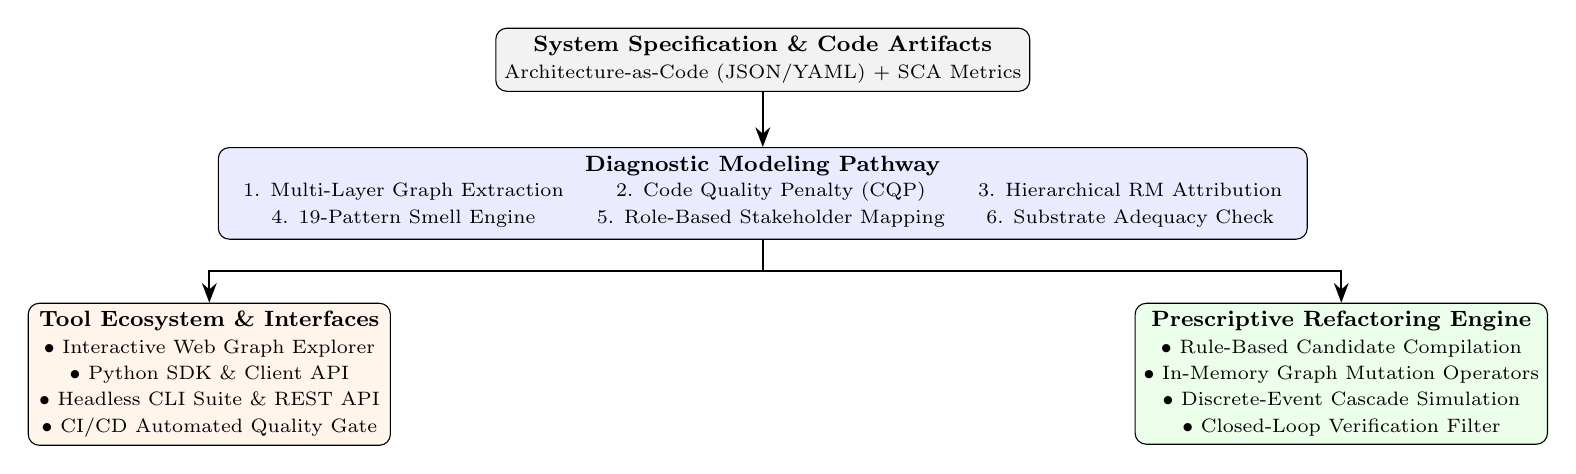
\begin{tikzpicture}[
    box/.style={draw, rounded corners, align=center, font=\footnotesize, inner sep=3pt},
    arr/.style={-{Stealth[length=2.5mm]}, thick},
    node distance=6mm and 8mm
]
\node[box, fill=gray!10, minimum width=4.5cm] (input) {
    \textbf{System Specification \& Code Artifacts} \\
    \scriptsize Architecture-as-Code (JSON/YAML) + SCA Metrics
};

\node[box, fill=blue!8, below=7mm of input, minimum width=8.5cm] (diag) {
    \textbf{Diagnostic Modeling Pathway} \\
    \begin{tabular}{c c c}
    \scriptsize 1. Multi-Layer Graph Extraction & \scriptsize 2. Code Quality Penalty (CQP) & \scriptsize 3. Hierarchical RM Attribution \\
    \scriptsize 4. 19-Pattern Smell Engine & \scriptsize 5. Role-Based Stakeholder Mapping & \scriptsize 6. Substrate Adequacy Check
    \end{tabular}
};

\node[box, fill=orange!8, below left=8mm and -22mm of diag, minimum width=4.6cm] (usability) {
    \textbf{Tool Ecosystem \& Interfaces} \\
    \scriptsize $\bullet$ Interactive Web Graph Explorer \\
    \scriptsize $\bullet$ Python SDK \& Client API \\
    \scriptsize $\bullet$ Headless CLI Suite \& REST API \\
    \scriptsize $\bullet$ CI/CD Automated Quality Gate
};

\node[box, fill=green!8, below right=8mm and -22mm of diag, minimum width=4.6cm] (presc) {
    \textbf{Prescriptive Refactoring Engine} \\
    \scriptsize $\bullet$ Rule-Based Candidate Compilation \\
    \scriptsize $\bullet$ In-Memory Graph Mutation Operators \\
    \scriptsize $\bullet$ Discrete-Event Cascade Simulation \\
    \scriptsize $\bullet$ Closed-Loop Verification Filter
};

\draw[arr] (input) -- (diag);
\draw[arr] (diag.south) -- ++(0,-4mm) -| (usability.north);
\draw[arr] (diag.south) -- ++(0,-4mm) -| (presc.north);
\end{tikzpicture}
\caption{System architecture of the Software-as-a-Graph (SaG) framework: the multi-layer graph metamodel and diagnostic pathway serve as the shared foundation powering both multi-modal tool interfaces (Web, SDK, CLI, CI/CD) and the closed-loop counterfactual refactoring engine.}
\label{fig:overview}
\end{figure}

\subsection{Target Audience and Tool Use Cases}
\label{sec:intro:audience}

SaG is designed to serve four primary categories of users in the systems and software modeling community:
\begin{enumerate}
    \item \textbf{Software and Systems Architects:} Architects use SaG to model event-driven topologies before deployment, visualize cross-layer dependency structures, detect architectural anti-patterns, and explore verified refactoring blueprints to eliminate structural bottlenecks.
    \item \textbf{Reliability and SRE Engineers:} Site reliability engineers leverage SaG's deterministic ISO 25010/25019 quality decompositions to identify Single Points of Failure and estimate blast-radius vulnerability without performing destructive fault-injection tests on production clusters.
    \item \textbf{MDE and Systems Modeling Researchers:} Researchers can utilize SaG as an extensible, open-source experimental platform for evaluating novel graph metrics, domain-specific anti-patterns, and model transformation algorithms on realistic distributed benchmarks.
    \item \textbf{DevOps and Quality Assurance Teams:} DevOps practitioners integrate SaG's headless CLI and regression gating protocols into continuous integration pipelines, preventing structural technical debt regressions before code merges.
\end{enumerate}

\subsection{Contributions to the Modeling Community}
\label{sec:intro:contributions}

In accordance with the criteria of the SoSyM Tool Paper Call, this article presents the following contributions:

\begin{enumerate}
    \item \textbf{A Domain-Specific Graph Metamodel for Publish--Subscribe Systems (Section~\ref{sec:sag_model}):} We formalize a typed, multi-layer multigraph metamodel ($V, E, \tau_V, \tau_E, w_V, w_E$) capturing applications, libraries, topics, brokers, and compute hosts across four layer projections, governed by seven formal dependency derivation rules and a continuous Code Quality Penalty (CQP).
    \item \textbf{A Formal Catalog of 19 Publish--Subscribe Anti-Patterns (Section~\ref{sec:antipattern_catalog}):} We formalize nineteen architectural anti-patterns stated over pub--sub constructs across Reliability, Availability, Maintainability, and Architecture, complete with metric signatures, adaptive box-plot detection thresholds, and finding scope classifications.
    \item \textbf{Tool Architecture and Implementation Techniques (Section~\ref{sec:tool_architecture}):} We detail SaG's hexagonal ports-and-adapters architecture, highlighting its dual-repository design pattern that pairs a persistent graph database (\texttt{Neo4jRepository}) with a high-throughput, in-memory sandboxed repository (\texttt{MemoryRepository}) enabling rapid counterfactual model transformations.
    \item \textbf{A Closed-Loop Counterfactual Refactoring Verifier (Section~\ref{sec:tool_architecture}):} We introduce a rule-based refactoring compiler coupled with three graph-mutation operators, implementing a two-level simulation verification discipline that rejects mutations failing to clear stochastic noise floor margins.
    \item \textbf{Tool Usability and Multi-Modal Interfaces (Section~\ref{sec:tool_usability}):} We describe the multi-modal interaction modalities engineered into SaG, including an interactive web-based graph explorer, a Python SDK, a modular CLI, a REST API, and CI/CD quality gating with standardized exit-code protocols.
    \item \textbf{Comprehensive Empirical Evaluation in Realistic Scenarios (Section~\ref{sec:empirical_application}):} We evaluate SaG across eight multi-domain benchmark scenarios (29 to 520 vertices) and three transcribed real-world open-source systems (Autoware.Universe, Apollo Cyber RT, and Cloud IoT Mesh), reporting ranking quality saturation (NDCG@10 $\approx 0.82$--$0.86$), catalog discrimination characteristics ($\kappa = +0.296$ on real-world topologies), and refactoring survival rates ($71.0\%$).
    \item \textbf{Community Importance and Lessons Learnt (Section~\ref{sec:community_and_lessons_learnt}):} In fulfillment of SoSyM's tool paper mandate, we explicitly articulate the framework's broader significance for systems modeling and detail five transferable lessons learnt across designing, building, testing, evaluating, and disseminating the tool.
    \item \textbf{Open-Source Availability and Reproducibility (Section~\ref{sec:discussion}):} The tool is released under the Apache 2.0 license, packaged for pip installation and Docker Compose deployment, and backed by a complete Zenodo-archived reproduction package with a persistent DOI.
\end{enumerate}

\subsection{Relationship to Prior Work}
\label{sec:intro:prior_work}

This paper builds upon and expands two prior research efforts by the authors:
\begin{enumerate}
    \item An initial conference workshop paper \citep{yigit2025graph} introduced an early prototype of the multi-layer graph representation and evaluated a preliminary heuristic criticality score ($CS$) against a reachability loss metric on a single, small 10-application system ($\rho = 0.94$). In Section~\ref{sec:empirical_application}, we re-measure this claim across eight heterogeneous scenarios under an independent discrete-event cascade simulator, explaining why ranking correlation on directed dependency graphs saturates around $\rho \approx 0.485$ and why deterministic, role-attributed quality modeling is the true value over scalar ranking.
    \item A companion research manuscript focuses specifically on a learned Graph Neural Network (GNN) predictor for blast-radius forecasting. The present tool paper is entirely distinct and self-contained: it presents the comprehensive \textbf{Software-as-a-Graph framework}, its domain metamodel, the formal 19-pattern catalog, the dual-repository architecture, the closed-loop counterfactual refactoring engine, the multi-modal tool interfaces, the realistic scenario evaluation, and the community lessons learnt.
\end{enumerate}

\subsection{Organization}
\label{sec:intro:org}

The remainder of this paper is structured as follows. Section~\ref{sec:related_work} reviews related work in MDE, architecture modeling, and smell detection. Section~\ref{sec:sag_model} defines the graph metamodel and diagnostic quality attribution framework. Section~\ref{sec:antipattern_catalog} details the 19-pattern anti-pattern catalog. Section~\ref{sec:tool_architecture} presents the tool architecture, implementation techniques, and counterfactual refactoring engine. Section~\ref{sec:tool_usability} describes tool usability, interfaces, and CI/CD integration. Section~\ref{sec:empirical_application} evaluates the tool on benchmark scenarios and real-world systems. Section~\ref{sec:community_and_lessons_learnt} articulates the tool's community importance and five key lessons learnt. Section~\ref{sec:discussion} addresses threats to validity and tool availability, and Section~\ref{sec:conclusion} concludes with future work.

\section{Background and Related Modeling Tools}
\label{sec:related_work}

\subsection{Model-Driven Engineering and Architectural Description Languages}
\label{sec:related:mde}

Model-Driven Engineering (MDE) elevates high-level system models to primary engineering artifacts, enabling automated analysis, formal verification, and code synthesis \citep{schmidt2006mde, combemale2016global}. Within software and systems modeling, Architecture Description Languages (ADLs) such as the Architecture Analysis \& Design Language (AADL) \citep{feiler2006aadl} and the Palladio Component Model (PCM) \citep{becker2009palladio} formalize structural hierarchies, component interfaces, and execution platforms for dependability and performance forecasting.

However, existing ADLs and architectural modeling tools are primarily tailored for synchronous remote procedure call (RPC), client--server interactions, or discrete hardware bus execution. In event-driven publish--subscribe (pub--sub) systems, communication is mediated through anonymous topics, message brokers, and Quality of Service (QoS) transport policies. Classical component-connector models fail to capture the subtle dynamic coupling introduced when dozens of subscribers bind to a single high-fanout topic or when broker memory partitions become exhausted under unthrottled producer bursts. SaG advances MDE by formalizing a domain-specific, typed multigraph metamodel specifically engineered to capture publish--subscribe topology semantics, multi-layer projections, and transport QoS contracts.

\subsection{Architectural Smell and Anti-Pattern Detection Tools}
\label{sec:related:smells}

In object-oriented software engineering, Fowler's refactoring catalog \citep{fowler1999refactoring} and Brown et al.'s AntiPatterns taxonomy \citep{brown1998antipatterns} formalized recurring design flaws and remediation strategies. Suryanarayana et al.\ systematized design smells using structural metrics \citep{suryanarayana2014refactoring}. In distributed microservices, Taibi et al.\ established empirical taxonomies of architectural smells, such as Cyclic Dependency, Shared Database, and Distributed Monolith \citep{taibi2020microservices}.

At the architectural level, automated smell detection is an established discipline. Mo et al.\ formalized architectural hotspots and evaluated their maintenance costs \citep{mo2015hotspot}. Specialized tools such as Arcan \citep{arcan2017}, Designite \citep{sharma2016designite}, and DV8 \citep{cai2019dv8} detect dependency smells from reverse-engineered source-code graphs, and recent surveys document their agreements and divergence \citep{azadi2019architectural, mumtaz2021systematic}. Common patterns such as cyclic dependencies, hub-like dependencies, and unstable interfaces align conceptually with \texttt{CYCLE}, \texttt{HUB\_AND\_SPOKE}, and \texttt{UNSTABLE\_INTERFACE} in our catalog.

However, existing tools operate on module, package, or class dependency graphs recovered from source code; \emph{they possess no representation for topics, message brokers, partition queues, or QoS transport policies}. Consequently, they are blind to the failure modes unique to publish--subscribe middleware. Furthermore, empirical studies by Lenarduzzi et al.\ \citep{lenarduzzi2020sonarqube} indicate that static rule-based tools (e.g., SonarQube) often exhibit weak correlation with real-world fault proneness. SaG addresses this by grounding its 19-pattern catalog in a multi-layer graph metamodel and evaluating detection against dynamic cascade simulation.

Software performance engineering has also cataloged performance antipatterns \citep{smith2000software, smith2002new}, which are detected in Java applications \citep{trubiani2023automated} or modeled via queueing networks \citep{pinciroli2023performance, avritzer2025architecture}. While patterns such as the Blob and One-Lane Bridge resemble SaG's \texttt{GOD\_COMPONENT} and \texttt{BROKER\_OVERLOAD}, they target execution latency, whereas SaG targets structural failure cascades. Similarly, scalability fault detectors (e.g., ScaleCheck \citep{stuardo2019scalecheck}, PCatch \citep{li2018pcatch}, and recent distributed fault studies \citep{zhu2026understanding}) target code-level thread and socket bottlenecks, whereas SaG targets pre-deployment architectural models.

\subsection{Model Refactoring: Open-Loop Search vs.\ Counterfactual Verification}
\label{sec:related:refactoring}

Automated model refactoring and architecture optimization have been approached through multiple modeling paradigms:
\begin{enumerate}
    \item \emph{Rule-Based Model Transformations:} Graph transformation tools apply declarative graph rewrite rules to restructure models based on predefined architectural patterns \citep{mens2006taxonomy}.
    \item \emph{Search-Based Software Engineering (SBSE):} Multi-objective evolutionary algorithms (e.g., NSGA-II) explore architectural design spaces to optimize coupling, cohesion, or hardware cost \citep{harman2012sbse, aleti2013software, deb2002fast}.
    \item \emph{Simulation-in-the-Loop Optimization:} The Palladio/PerOpteryx line of work \citep{koziolek2011peropteryx} evaluates candidate architectural variants within an optimization loop using simulation and analytical models.
\end{enumerate}

Despite these advances, the vast majority of architectural refactoring engines operate \emph{open-loop} with respect to failure propagation: transformations are selected either by heuristic structural fitness functions or by unverified rule triggers. SaG introduces a closed-loop \textbf{``verify-before-transform''} discipline: candidate graph mutations are executed in an in-memory sandbox and evaluated against a discrete-event cascade simulator across multiple seeds and failure thresholds. Edits are admitted only if the measured impact reduction clears stochastic seed noise ($\overline{\Delta I} > \kappa \sigma_{\text{seed}}$), preventing regressions.

\subsection{Explainable Quality Models and Graph Centrality}
\label{sec:related:quality_models}

Software quality models, standardized in ISO/IEC 25010 (Product Quality) and ISO/IEC 25019 (Quality-in-Use) \citep{iso25010_2023, iso25019_2023}, structure software quality into hierarchical characteristics. In distributed systems, however, predictive analytics often rely on opaque machine learning models or collapse multiple metrics into unweighted sums \citep{menzies2018bad}.

SaG strictly distinguishes \emph{post-hoc attribution} (e.g., SHAP or GNN attention weights, which approximate an opaque model's decisions) from \emph{intrinsic score decomposition}. SaG defines its Reliability--Maintainability (RM) quality model as a deterministic, weighted decomposition over standardized sub-characteristics (Fault Tolerance, Availability, Maintainability). This ensures that every computed score has auditable provenance directly mapped to stakeholder engineering roles.

Finally, while complex network theory applies graph centrality indices (betweenness \citep{freeman1977set}, degree, PageRank, articulation points) to microservices and call graphs \citep{bakhtin2025network, falci2018complex}, our empirical evaluation reveals that multi-dimensional metrics saturate at comparable ranking accuracy with degree centrality (Section~\ref{sec:empirical_application}). SaG's principal value is therefore its deterministic, domain-grounded attribution and verified refactoring, rather than superior scalar ranking.

\subsection{Advance Over State of the Art}
\label{sec:related:sota}

Table~\ref{tab:sota_comparison} summarizes SaG's key contributions in comparison to state-of-the-art modeling and architecture analysis tools.

\begin{table}[htbp]
\centering
\footnotesize
\setlength{\tabcolsep}{3.5pt}
\caption{Comparison of SaG with State-of-the-Art Modeling and Architecture Tools.}
\label{tab:sota_comparison}
\begin{tabularx}{\textwidth}{lccccc}
\toprule
\textbf{Capability / Characteristic} & \textbf{Palladio / PerOpteryx} & \textbf{AADL} & \textbf{Arcan / Designite} & \textbf{SonarQube} & \textbf{SaG (This Tool)} \\
\midrule
Pub--Sub Semantics (Topics, Brokers, QoS) & No & Partial & No & No & \textbf{Yes (First-Class)} \\
Multi-Layer Heterogeneous Metamodel & Component/Hardware & Component/Bus & Class/Package & File/Line & \textbf{Yes (4 Layers, 5 Types)} \\
Standardized Quality Model & Custom metrics & Custom annexes & Smells only & Technical Debt & \textbf{ISO/IEC 25010 \& 25019} \\
Domain-Specific Anti-Pattern Catalog & Performance only & Fault trees & OO / Microservices & Code rules & \textbf{19 Pub--Sub Patterns} \\
Code-to-Architecture Bridge (CQP) & No & No & No & Native (AST) & \textbf{Yes (Continuous CQP)} \\
Refactoring Verification Discipline & Open-loop / Sim & Analytic / Open & Open-loop & Advisory only & \textbf{Closed-Loop Simulation} \\
In-Memory Sandboxed Transformation & No & No & No & No & \textbf{Yes (\texttt{MemoryRepository})} \\
Multi-Modal Interfaces (Web, SDK, CLI) & Eclipse IDE & OSATE / Eclipse & CLI / Desktop & Web Dashboard & \textbf{Web, SDK, CLI, REST} \\
CI/CD Regression Quality Gating & No & No & Partial & Yes & \textbf{Yes (3-Tier Exit Codes)} \\
Open Source License & EPL & Open source & Proprietary/Academic & LGPL / Freemium & \textbf{Apache 2.0 (Open)} \\
\bottomrule
\end{tabularx}
\end{table}

\section{Graph Metamodel and Multi-Layer System Representation}
\label{sec:sag_model}

\subsection{Heterogeneous Graph Metamodel}
\label{sec:model:formulation}

In the SaG framework, a distributed publish--subscribe software architecture is formalized as a typed, attributed, directed multigraph:
\begin{equation}
G = (V, E, \tau_V, \tau_E, w_E, w_V)
\end{equation}
where $V$ is the set of architectural vertices, $E \subseteq V \times V$ is the multiset of directed edges, $\tau_V : V \to T_V$ partitions vertices into five distinct semantic classes, $\tau_E : E \to T_E$ assigns each edge to an architectural relationship type, $w_E : E \to \mathbb{R}^+$ maps edges to QoS-derived communication weights, and $w_V : V \to [0,1]$ assigns normalized component weights.

The vertex type universe $T_V$ captures the fundamental building blocks of publish--subscribe architectures:
\begin{equation}
T_V = \{\text{Application}, \text{Library}, \text{Topic}, \text{Broker}, \text{Node}\}
\end{equation}
\begin{itemize}
    \item \textbf{Application ($V_{\text{app}}$):} Autonomous execution processes (e.g., ROS~2 nodes, microservice daemons) that actively produce or consume messages.
    \item \textbf{Library ($V_{\text{lib}}$):} Passive shared code modules or algorithmic libraries dynamically or statically linked by applications.
    \item \textbf{Topic ($V_{\text{topic}}$):} Named publish--subscribe communication channels routing asynchronous message streams.
    \item \textbf{Broker ($V_{\text{broker}}$):} Message routing and queuing intermediaries (e.g., MQTT brokers, Kafka partition leaders, DDS domain participants).
    \item \textbf{Node ($V_{\text{node}}$):} Physical or virtual compute hosts, containers, or virtual machines executing processes and brokers.
\end{itemize}

The edge type universe $T_E$ formalizes the operational and structural relationships among these entities:
\begin{equation}
\begin{split}
T_E = \{ & \text{PUBLISHES\_TO}, \text{SUBSCRIBES\_TO}, \text{ROUTES}, \\
        & \text{RUNS\_ON}, \text{CONNECTS\_TO}, \text{USES}\}
\end{split}
\end{equation}

\subsection{Derived Architectural Dependencies: The \texttt{DEPENDS\_ON} Projection}
\label{sec:model:projection}

Because pub--sub systems achieve spatial and temporal decoupling via topic mediation, direct runtime invocation dependencies are not explicitly declared in source manifests. To expose indirect failure propagation pathways, SaG defines formal derivation rules that project $G$ into a directed analysis graph $G_{\text{analysis}} = (V, E_{\text{depends}})$, where directed edges $(u \to v)$ denote that entity $u$ functionally depends on entity $v$ (i.e., disruption of $v$ directly impacts $u$):

\begin{itemize}
    \item \textbf{Application-to-Application:} Formed when application $A_1$ subscribes to a topic $T$ published by application $A_2$: $(A_1 \to A_2) \in E_{\text{depends}}$.
    \item \textbf{Application-to-Broker:} Formed when application $A$ publishes or subscribes to a topic routed through broker $B$: $(A \to B) \in E_{\text{depends}}$.
    \item \textbf{Application-to-Library:} Formed when application $A$ links shared library $L$: $(A \to L) \in E_{\text{depends}}$, capturing shared-dependency blast radius if $L$ suffers a defect.
    \item \textbf{Broker-to-Broker / Node Colocation:} Captures shared-fate host vulnerabilities when multiple critical applications or brokers are co-located on the same physical host $N$: $(A_i \to N) \in E_{\text{depends}}$.
\end{itemize}

The resulting analysis graph is stratified across four architectural layer projections:
\begin{enumerate}
    \item \textbf{Application Layer ($\text{app}$):} Subgraph induced by $V_{\text{app}} \cup V_{\text{lib}}$, modeling end-to-end business logic and functional data flows.
    \item \textbf{Infrastructure Layer ($\text{infra}$):} Subgraph induced by $V_{\text{node}}$, modeling physical and virtual compute network topology.
    \item \textbf{Middleware Layer ($\text{mw}$):} Subgraph induced by $V_{\text{app}} \cup V_{\text{broker}}$, modeling broker mediation, partition bottlenecks, and transport queues.
    \item \textbf{System Layer ($\text{system}$):} The complete multi-layer graph across all five vertex types, capturing cross-layer failure cascades.
\end{enumerate}

\subsection{The Code Quality Penalty (CQP): Bridging SCA and Architecture}
\label{sec:model:cqp}

To bridge source-level implementation health with macro-architectural risk, SaG ingests four file-level static code analysis (SCA) metrics for Application and Library components:
\begin{itemize}
    \item Total Lines of Code (\texttt{loc}, sizing component scale),
    \item Average Weighted Methods per Class (\texttt{cyclomatic\_complexity}, proxy for cognitive complexity),
    \item Lack of Cohesion in Methods (\texttt{lcom}, proxy for modularity decay),
    \item Code-level instability, $\text{instability\_code}(v) = C_e(v) / (C_a(v) + C_e(v))$, computed from efferent and afferent coupling.
\end{itemize}

Signals are min-max normalized independently within each component type population (Applications and Libraries form distinct populations with different scale baselines). Populations with zero variance collapse to $0$ rather than $1$, ensuring that absent data is not penalized as worst-case debt. These normalized metrics synthesize into the continuous \textbf{Code Quality Penalty (CQP)}:
\begin{equation}
\begin{aligned}
\mathrm{CQP}(v) = & \; 0.10\,\text{loc\_norm}(v) + 0.35\,\text{complexity\_norm}(v) \\
                  & + 0.30\,\text{instability\_code}(v) + 0.25\,\text{lcom\_norm}(v)
\end{aligned}
\end{equation}
$\mathrm{CQP}(v) \in [0,1]$ provides an explicit, quantitative bridge from source-code technical debt to architectural criticality, entering directly into the Maintainability dimension of the quality model.

\subsection{Hierarchical Reliability--Maintainability (RM) Quality Model}
\label{sec:model:rm}

Grounded in \textbf{ISO/IEC 25010} (Product Quality) and \textbf{ISO/IEC 25019} (Quality-in-Use) \citep{iso25010_2023, iso25019_2023}, SaG decomposes architectural quality into two primary dimensions---\textbf{Reliability} and \textbf{Maintainability}---providing explainable, role-specific diagnostics (Figure~\ref{fig:rm_hierarchy}, Table~\ref{tab:rm_stakeholders}).

\begin{figure}[htbp]
\centering
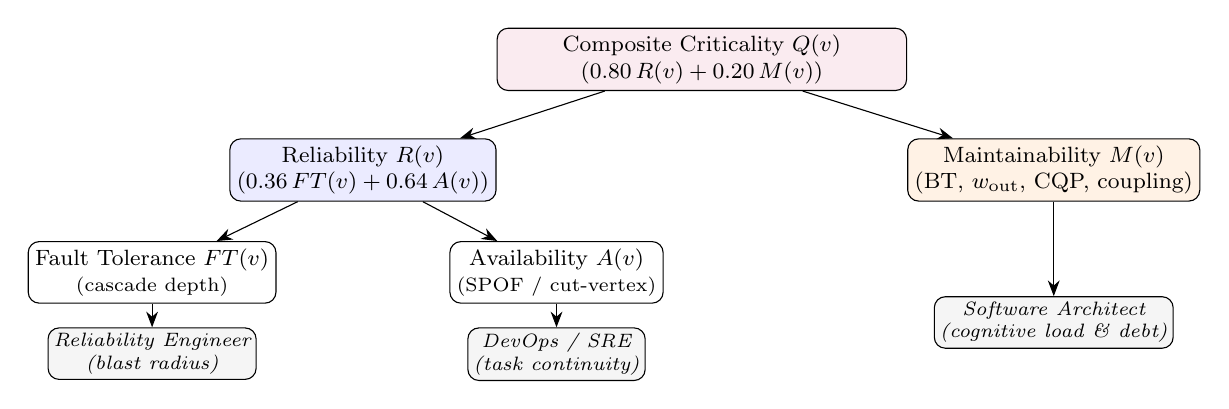
\begin{tikzpicture}[
    box/.style={draw, rounded corners, align=center, font=\footnotesize, inner sep=2.5pt},
    role/.style={draw, rounded corners, align=center, font=\scriptsize\itshape, fill=gray!8, inner sep=2pt},
    >={Stealth[length=2mm]}, node distance=5mm and 5mm
]
\node[box, fill=purple!8, minimum width=5.2cm] (q) {Composite Criticality $Q(v)$ \\ $(0.80\,R(v) + 0.20\,M(v))$};
\node[box, fill=blue!8, below left=6mm and 0mm of q, minimum width=3.0cm] (r) {Reliability $R(v)$ \\ $(0.36\,FT(v) + 0.64\,A(v))$};
\node[box, fill=orange!10, below right=6mm and 0mm of q, minimum width=3.0cm] (m) {Maintainability $M(v)$ \\ (BT, $w_{\text{out}}$, CQP, coupling)};
\node[box, below left=5mm and -6mm of r, minimum width=1.7cm] (ft) {Fault Tolerance $FT(v)$ \\ \scriptsize (cascade depth)};
\node[box, below right=5mm and -6mm of r, minimum width=1.7cm] (a) {Availability $A(v)$ \\ \scriptsize (SPOF / cut-vertex)};
\node[role, below=3mm of ft] (rft) {Reliability Engineer \\ (blast radius)};
\node[role, below=3mm of a] (ra) {DevOps / SRE \\ (task continuity)};
\node[role, below=12mm of m] (rm) {Software Architect \\ (cognitive load \& debt)};
\draw[->] (q) -- (r);
\draw[->] (q) -- (m);
\draw[->] (r) -- (ft);
\draw[->] (r) -- (a);
\draw[->] (ft) -- (rft);
\draw[->] (a) -- (ra);
\draw[->] (m) -- (rm);
\end{tikzpicture}
\caption{The hierarchical RM Diagnostic Attribution Model and stakeholder role mapping. Each arrow represents a deterministic scoring dependency computed in a single pass.}
\label{fig:rm_hierarchy}
\end{figure}

\begin{table}[htbp]
\centering
\small
\setlength{\tabcolsep}{4pt}
\caption{RM Quality Dimensions, Stakeholder Roles, and ISO/IEC 25019 Quality-in-Use Mapping.}
\label{tab:rm_stakeholders}
\begin{tabularx}{\textwidth}{l>{\raggedright\arraybackslash}p{2.6cm}>{\raggedright\arraybackslash}p{2.4cm}X>{\raggedright\arraybackslash}p{2.4cm}}
\toprule
\textbf{Dim.} & \textbf{Sub-Characteristic} & \textbf{Engineering Role} & \textbf{High Score Meaning} & \textbf{ISO 25019 Harm} \\
\midrule
\textbf{R} & \textbf{Fault Tolerance ($FT$)} & Reliability Engineer & Cascades deeply; large blast radius & Indirect Harm \\
& \textbf{Availability ($A$)} & DevOps / SRE & Single point of failure; partition & Primary Task Loss \\
\textbf{M} & Structural Coupling & Software Architect & High change ripple; code-level debt & Maintainer Effort \\
\bottomrule
\end{tabularx}
\end{table}

\paragraph{Formal Quality Definitions.}
\begin{itemize}
    \item \textbf{Definition D1 (Component Criticality):} Let $G_l = (V_l, E_l)$ be a layer-projected graph. Component criticality $\mathrm{crit}_l : V_l \to [0,1]^2 \times [0,1]$ maps vertex $v$ to metric vector $\mathbf{s}(v) = [R(v), M(v)]^T$ and composite score $Q(v)$, estimating Quality-in-Use degradation.
    \item \textbf{Definition D2 (Relationship Criticality):} Let $e = (u,v) \in E_l$ be a dependency edge. Relationship criticality $\mathrm{crit}_l(e) \in [0,1]$ estimates Quality-in-Use loss resulting from link disruption.
    \item \textbf{Definition D3 (Consequence Metric):} Criticality measures structural consequence given failure. Failure likelihood is supplied externally from operational telemetry.
    \item \textbf{Definition D4 (Relative Distribution):} Criticality classifications are relative to the score distribution of system $S$ at layer $l$.
\end{itemize}

\paragraph{Structural Inputs.}
Let $\varepsilon = 10^{-9}$. The model computes the following structural metrics on $G_l$:
\begin{itemize}
    \item $\mathrm{RPR}(v)$: PageRank on the transposed graph $G_l^{\mathsf T}$, rank-normalized over the population. Because \texttt{DEPENDS\_ON} edges point dependent~$\to$~dependency, failure propagates \emph{against} edge direction; reverse PageRank is thus the true cascade-reach estimator.
    \item $\mathrm{DG}_{\text{in}}(v) = \deg^{-}(v) / (|V_l| - 1)$ and $\mathrm{DG}_{\text{out}}(v) = \deg^{+}(v) / (|V_l| - 1)$.
    \item \textbf{Multi-Path Coupling Index:} $\mathrm{MPCI}(v) = \sum_{e \in \mathrm{In}(v)} \max(\mathrm{paths}(e) - 1,\, 0) \,/\, (|V_l| - 1)$, where $\mathrm{paths}(e)$ counts distinct pub--sub channels realizing dependency $e$.
    \item \textbf{Fan-Out Criticality} (Topic vertices): $\mathrm{FOC}(t) = \ln(1 + f(t))\, s(t) \,/\, \max_{t'} [\ln(1 + f(t'))\, s(t')]$, for publication frequency $f(t)$ in Hz and subscriber count $s(t)$.
    \item \textbf{Directed Articulation Score:} $\mathrm{AP}_{c,\text{directed}}(v) = \max(\mathrm{AP}_c^{\text{out}}(v), \mathrm{AP}_c^{\text{in}}(v))$, where $\mathrm{AP}_{c}^{\text{out}}(v) = 1 - L(G_l \setminus \{v\})/(|V_l|-1)$ and $L(H)$ is the order of the largest connected component of $H$.
    \item \textbf{Bridge Ratio:} $\mathrm{BR}(v) = |\{e \in \mathrm{bridges}(G_l^{\text{und}}) : v \in e\}| / \deg^{\text{und}}(v)$.
    \item \textbf{Connectivity Degradation Index:} $\mathrm{CDI}(v) = \min\!\big( [\bar{d}(G_l \setminus \{v\}) - \bar{d}(G_l)] / \bar{d}(G_l),\; 1 \big)$, for $\bar{d}$ the average shortest-path length over reachable pairs.
    \item $\mathrm{BT}(v)$: betweenness centrality; $\mathrm{CC}(v)$: clustering coefficient; $\mathrm{PC}(v)$: normalized path complexity; $w(v)$: normalized QoS component weight; $w_{\text{out}}(v)$: normalized summed efferent QoS weight.
\end{itemize}

\paragraph{Mathematical Formulation of Quality Dimensions.}
\begin{enumerate}
    \item \textbf{Fault Tolerance ($FT$).} Estimates cascade reach. For Application, Library, Broker, and Node vertices, an enhanced cascade-depth potential $\mathrm{CDPot}$ discounts vertices that forward more than they absorb, amplified by multi-path coupling:
    \begin{equation}
    \begin{aligned}
    \mathrm{CDPot}_{\text{base}}(v) &= \frac{\mathrm{RPR}(v) + \mathrm{DG}_{\text{in}}(v)}{2}\left(1 - \min\!\left(\frac{\deg^{+}(v)}{\max(\deg^{-}(v),\varepsilon)},\, 1\right)\right) \\
    \mathrm{CDPot}(v) &= \min\!\big(\mathrm{CDPot}_{\text{base}}(v)\,(1 + \mathrm{MPCI}(v)),\; 1\big) \\
    FT(v) &= 0.45\,\mathrm{RPR}(v) + 0.30\,\mathrm{DG}_{\text{in}}(v) + 0.25\,\mathrm{CDPot}(v)
    \end{aligned}
    \end{equation}
    For Topic vertices, the blast surface is the subscriber set moderated by publisher redundancy:
    \begin{equation}
    FT_{\text{topic}}(t) = 0.50\,\mathrm{FOC}(t) + 0.50\,\mathrm{FOC}(t)\big(1 - \min(w_{\text{in}}(t), 1)\big)
    \end{equation}
    \item \textbf{Availability ($A$).} Evaluates single-point-of-failure exposure. The interaction term $\mathrm{QSPOF}(v) = \mathrm{AP}_{c,\text{directed}}(v)\cdot w(v)$ deliberately incorporates QoS weight so structural SPOF risk is not masked at low weight:
    \begin{equation}
    \begin{aligned}
    A(v) = & \; 0.25\,\mathrm{AP}_{c,\text{directed}}(v) + 0.20\,\mathrm{QSPOF}(v) \\
           & + 0.20\,\mathrm{BR}(v) + 0.25\,\mathrm{CDI}(v) + 0.10\,w(v)
    \end{aligned}
    \end{equation}
    \item \textbf{Maintainability ($M$).} Blends betweenness, efferent QoS out-degree, CQP, coupling risk, and inverse clustering. With $\iota(v) = \deg^{+}(v) / (\deg^{-}(v) + \deg^{+}(v) + \varepsilon)$:
    \begin{equation}
    \begin{aligned}
    \mathrm{CouplingRisk\_enh}(v) &= \min\!\big(1,\; \big[1 - |2\iota(v) - 1|\big]\,(1 + 0.10\,\mathrm{PC}(v))\big) \\
    M(v) = & \; 0.35\,\mathrm{BT}(v) + 0.30\,w_{\text{out}}(v) + 0.15\,\mathrm{CQP}(v) \\
           & + 0.12\,\mathrm{CouplingRisk\_enh}(v) + 0.08\,(1-\mathrm{CC}(v))
    \end{aligned}
    \end{equation}
    \item \textbf{Reliability Composite ($R$).} Blends Fault Tolerance and Availability with $\alpha = 0.36$:
    \begin{equation}
    R(v) = \alpha \cdot FT(v) + (1-\alpha) \cdot A(v)
    \end{equation}
\end{enumerate}

\paragraph{Composite Criticality and Stakeholder Projection.}
Composite criticality blends Reliability and Maintainability:
\begin{equation}
Q(v) = 0.80\,R(v) + 0.20\,M(v)
\end{equation}
The diagnostic vector $\mathbf{s}_{\text{RM}}(v) = [R(v), M(v)]^T$ projects into ISO/IEC 25019 Quality-in-Use stakeholder harm scores $[H_{\text{Ben}}, H_{\text{Risk}}, H_{\text{Acc}}]^T$ via transformation matrix $\mathbf{M}_{\text{RM} \to \text{QiU}}$:
\begin{equation}
\mathbf{h}_{\text{QiU}}(v) = \mathbf{M}_{\text{RM} \to \text{QiU}} \cdot \mathbf{s}_{\text{RM}}(v) = \begin{bmatrix} 0.75 & 0.25 \\ 0.80 & 0.20 \\ 0.60 & 0.40 \end{bmatrix} \begin{bmatrix} R(v) \\ M(v) \end{bmatrix}
\end{equation}
$\mathbf{M}_{\text{RM} \to \text{QiU}}$ is row-stochastic, providing a declared re-presentation of RM in stakeholder-facing terms for routing findings to responsible engineering roles. Components are classified into five severity tiers (\texttt{CRITICAL}, \texttt{HIGH}, \texttt{MEDIUM}, \texttt{LOW}, \texttt{MINIMAL}) using adaptive box-plot fences ($Q > Q_3 + 1.5\,\mathrm{IQR}$ for \texttt{CRITICAL}; $Q_3 < Q \le \text{fence}$ for \texttt{HIGH}).

\subsection{Substrate Adequacy: Layer Requirements for Topological Metrics}
\label{sec:model:substrate}

A foundational insight of our metamodel is that architectural quality dimensions are not equally well-posed on all layer projections. Continuous metrics ($FT$ and $M$) vary smoothly across all layers. In contrast, discrete cut-vertex and bridge predicates ($\mathrm{AP}_{c,\text{directed}}$ and $\mathrm{BR}$ in Availability) fire only where the projected graph contains cut vertices. 

On densely interconnected application-layer projections where topics allow multiple redundant paths, cut structures can be structurally absent ($F_1 = 0.0$ for articulation-point detection). Because $A(v)$ carries $(1-\alpha) = 0.64$ of $R(v)$'s weight, an availability score evaluated on an inadequate substrate collapses to a near-constant baseline. Substrate adequacy is therefore a design-time property: Availability-focused analysis (such as SPOF detection) must be evaluated on layer projections where physical or mediation bottlenecks exist---specifically the Middleware or System layers.

\section[Architectural Anti-Pattern Catalog for Publish--Subscribe Systems]{A Catalog of Architectural Anti-Patterns for\\ Publish--Subscribe Systems}
\label{sec:antipattern_catalog}

\subsection{Architectural Anti-Patterns vs.\ Smells in Systems Modeling}
\label{sec:catalog:taxonomy}

In model-based systems engineering, structural quality findings fall into two primary confidence tiers:
\begin{itemize}
    \item \textbf{Architectural Anti-Pattern:} A proven structural pathology known to cause systemic vulnerability or failure cascades under message bursts, requiring model-level architectural refactoring (e.g., Single Point of Failure, God Component, Broker Overload).
    \item \textbf{Architectural Bad Smell:} A localized topological anomaly signaling potential maintainability or reliability degradation, warranting architectural inspection (e.g., Chatty Pair, QoS Mismatch, Orphaned Topic).
\end{itemize}

Publish--subscribe architectural anomalies leave distinct \textbf{topological signatures} in the dependency graph. Because these signatures are directly computable from static architectural models, SaG detects them early in the design lifecycle before deployment on physical target clusters.

\subsection{Detection Methodology}
\label{sec:catalog:methodology}

Detection operates over fourteen structural metrics derived from $G_{\text{analysis}}$: Reverse PageRank ($\mathrm{RPR}$), in-degree and out-degree ($\mathrm{DG}_{\text{in}}$, $\mathrm{DG}_{\text{out}}$), multi-path coupling index ($\mathrm{MPCI}$), topic fan-out criticality ($\mathrm{FOC}$), betweenness centrality ($\mathrm{BT}$), QoS-weighted in- and out-degree ($w_{\text{in}}$, $w_{\text{out}}$), clustering coefficient ($\mathrm{CC}$), path complexity ($\mathrm{PC}$), directed articulation score ($\mathrm{AP}_{c,\text{directed}}$), bridge ratio ($\mathrm{BR}$), connectivity degradation index ($\mathrm{CDI}$), and component weight ($w$)---plus the synthesized Code Quality Penalty ($\mathrm{CQP}$, Section~\ref{sec:model:cqp}). This yields fifteen continuous metrics evaluated against adaptive box-plot fences ($Q_3 + k\,\mathrm{IQR}$, parameterized with $k=1.5$).

\subsection{Catalog Overview}
\label{sec:catalog:overview}

Table~\ref{tab:antipattern_catalog} summarizes the nineteen formal anti-patterns across three severity tiers, four quality categories, and four finding scopes: \textbf{Component} (attributed to a single vertex), \textbf{Edge} (attributed to a directed relationship), \textbf{Pair} (attributed to a bidirectional component pair), and \textbf{System} (a global topology characteristic).

\begin{table}[htbp]
\centering
\scriptsize
\setlength{\tabcolsep}{2.5pt}
\caption{Publish--Subscribe Architectural Anti-Pattern and Bad Smell Catalog. \textbf{Trig.} marks patterns that fire at least once on the eight-scenario benchmark corpus (Section~\ref{sec:catalog:coverage}).}
\label{tab:antipattern_catalog}
\begin{tabularx}{\textwidth}{>{\raggedright\arraybackslash}p{2.7cm}lll>{\raggedright\arraybackslash}X>{\raggedright\arraybackslash}p{2.6cm}c}
\toprule
\textbf{Pattern} & \textbf{Sev.} & \textbf{Category} & \textbf{Scope} & \textbf{Detection Signal} & \textbf{Autom. Refactoring} & \textbf{Trig.} \\
\midrule
\texttt{SPOF} & CRITICAL & Availability & Component & Articulation point $\wedge$ QoS SPOF score & Anti-affinity reallocation & \checkmark \\
\texttt{SYSTEMIC\_RISK} & CRITICAL & Reliability & System & Share of CRITICAL components $> 20\%$ & Advisory & \\
\texttt{CYCLE} & HIGH & Architecture & System & Strongly connected component / loop & Advisory & \checkmark \\
\texttt{GOD\_COMPONENT} & CRITICAL & Maintainability & Component & Extreme betweenness $\wedge$ CRITICAL $M(v)$ & Logical topic splitting & \\
\texttt{BOTTLENECK\_EDGE}& HIGH & Availability & Edge & Edge betweenness centrality outlier & Logical topic splitting & \checkmark \\
\texttt{BROKER\_OVERLOAD} & HIGH & Availability & Component & Broker availability $\ge 2\times$ median load & Anti-affinity reallocation & \\
\texttt{DEEP\_PIPELINE} & HIGH & Reliability & System & Path length $\ge \max(5, P_{75})$ & Advisory & (excl.) \\
\texttt{TOPIC\_FANOUT} & MEDIUM & Reliability & Component & Topic subscriber out-degree outlier & Logical topic splitting & \\
\texttt{CHATTY\_PAIR} & MEDIUM & Maintainability & Pair & Bidirectional weight product $> \tau_{\text{chatty}}$ & Advisory & \\
\texttt{QOS\_MISMATCH} & MEDIUM & Reliability & Edge & Pub/Sub QoS-weight gap $> \tau_{\text{qos}}$ & Advisory (Manual / Relay) & \checkmark \\
\texttt{ORPHANED\_TOPIC}& MEDIUM & Maintainability & Component & Zero in- or out-degree on graph & Advisory & \\
\texttt{UNSTABLE\_INTERFACE}& MEDIUM & Maintainability & Component & High \texttt{CouplingRisk\_enh} $\wedge$ high $M(v)$ & Advisory & \checkmark \\
\texttt{BRIDGE\_EDGE} & HIGH & Availability & Edge & Graph-theoretic bridge cut-edge & Advisory & \checkmark \\
\texttt{FAILURE\_HUB} & CRITICAL & Reliability & Component & Reliability outlier $\wedge$ high out-degree & Logical topic splitting & \\
\texttt{CONCENTRATION\_RISK}& MEDIUM & Reliability & System & Top-3 PageRank share $> 0.50$ & Advisory & \\
\texttt{HUB\_AND\_SPOKE} & MEDIUM & Maintainability & Component & Low clustering $\wedge$ degree $> 3$ & Logical topic splitting & \checkmark \\
\texttt{CHAIN} & MEDIUM & Architecture & System & Degree-bounded linear subgraph & Advisory & \\
\texttt{ISOLATED} & MEDIUM & Architecture & Component & Zero total degree & Advisory & \checkmark \\
\texttt{COMPOUND\_RISK} & CRITICAL & Architecture & Component & Co-occurring SPOF + God/Hub finding & Anti-affinity reallocation & \\
\bottomrule
\end{tabularx}
\end{table}

\subsection{Representative Pattern Walkthroughs}
\label{sec:catalog:walkthroughs}

\begin{enumerate}
    \item \textbf{SPOF (Single Point of Failure):} A component whose removal disconnects the graph ($\mathrm{AP}_{c,\text{directed}}(v) > 0$). Detection combines graph connectivity testing with QoS weighting ($\mathrm{QSPOF}(v) = \mathrm{AP}_c(v) \times w(v)$). Remediation generates host anti-affinity constraints.
    \item \textbf{GOD\_COMPONENT:} An application exhibiting extreme betweenness and CRITICAL maintainability ($\mathrm{BT}(v) > 0.30 \wedge M(v) \in \text{CRITICAL}$). Remediation decomposes pub--sub channels via logical topic splitting.
    \item \textbf{BROKER\_OVERLOAD (Cautionary Benchmark Case):} A broker routing $\ge 2\times$ the median broker's traffic. \emph{Cautionary finding:} In scenario S05 (two equally overloaded brokers), the within-population relative median rule cannot fire because each broker \emph{is} the median, demonstrating the necessity of absolute capacity-aware thresholds.
    \item \textbf{CHATTY\_PAIR:} Two components maintaining bidirectional high-frequency dependencies across separate topics ($(u \to v) \wedge (v \to u)$), representing tight coupling masquerading as pub--sub decoupling.
    \item \textbf{QOS\_MISMATCH:} A publisher offering weaker reliability than the subscriber requires ($w_{\text{pub}}(u) < w_{\text{sub}}(v) - \tau$). In DDS/ROS~2, this produces silent connection drops at runtime without compile-time errors.
\end{enumerate}

\subsection{Detection Validation Methodology}
\label{sec:catalog:validation}

Detection accuracy is validated against an independent discrete-event cascade simulation oracle ($I_{\text{comp}}(v)$) that models cascading message dropouts and queue exhaustion under component removal.

\subsection{Catalog Coverage on the Benchmark Corpus}
\label{sec:catalog:coverage}

Across all eight benchmark scenarios, \texttt{DEEP\_PIPELINE} is excluded due to path enumeration complexity (Section~\ref{sec:results:performance}), and of the remaining eighteen active detectors, \textbf{eight trigger at least one finding} on this corpus (Table~\ref{tab:antipattern_catalog}, \textbf{Trig.} column): Bottleneck Dependency (\texttt{BOTTLENECK\_EDGE}, 4974 findings), QoS Policy Mismatch (\texttt{QOS\_MISMATCH}, 1243), Unstable Interface (64), SPOF (17), Hub-and-Spoke (14), Dependency Cycle (\texttt{CYCLE}, 9), Bridge Edge (5), and Isolated Component (3). The remaining ten active patterns are fully unit-tested but require specific architectural topologies not present in these synthetic generators.

Crucially, of the 6329 total findings, only \textbf{98 ($1.5\%$)} are directly component-scoped (SPOF 17, Unstable Interface 64, Isolated Component 3, Hub-and-Spoke 14); the remaining \textbf{6231 ($98.4\%$)} are Edge- or System-scoped (dominated by Bottleneck Dependency and QoS Mismatches). This scope distribution explains the catalog's component-implication rate: edge-scoped findings implicate components as endpoints, resulting in broad screening sensitivity.

\section{Tool Architecture and Implementation Techniques}
\label{sec:tool_architecture}

\subsection{Hexagonal Ports-and-Adapters Architecture and Dual-Repository Design}
\label{sec:tool:hexagonal}

To decouple domain modeling and verification algorithms from underlying storage technologies, SaG is implemented according to a \textbf{hexagonal (ports-and-adapters) architecture} \citep{martin2003agile}. As illustrated in Figure~\ref{fig:hexagonal_arch}, core modeling services interact with graph storage exclusively through an abstract port interface, \texttt{IGraphRepository}.

\begin{figure}[htbp]
\centering
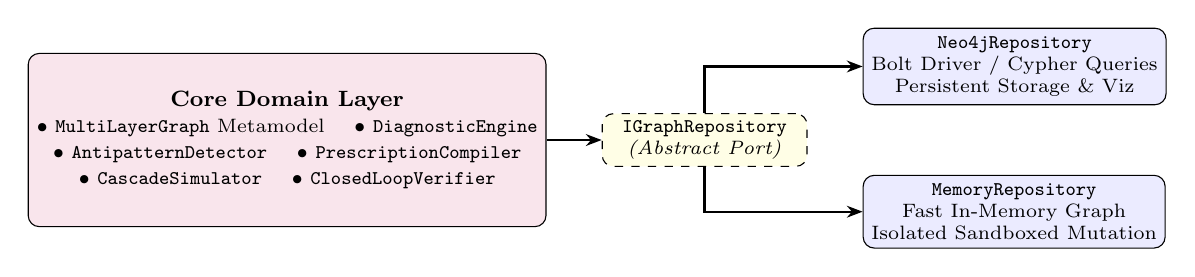
\begin{tikzpicture}[
    box/.style={draw, rounded corners, align=center, font=\footnotesize, inner sep=3pt},
    port/.style={draw, dashed, rounded corners, fill=yellow!10, align=center, font=\scriptsize, inner sep=2.5pt},
    adapter/.style={draw, rounded corners, fill=blue!8, align=center, font=\scriptsize, inner sep=3pt},
    arr/.style={-{Stealth[length=2mm]}, thick},
    node distance=5mm and 6mm
]
\node[box, fill=purple!10, minimum width=6.5cm, minimum height=2.2cm] (core) {
    \textbf{Core Domain Layer} \\
    \scriptsize $\bullet$ \texttt{MultiLayerGraph} Metamodel \quad $\bullet$ \texttt{DiagnosticEngine} \\
    \scriptsize $\bullet$ \texttt{AntipatternDetector} \quad $\bullet$ \texttt{PrescriptionCompiler} \\
    \scriptsize $\bullet$ \texttt{CascadeSimulator} \quad $\bullet$ \texttt{ClosedLoopVerifier}
};

\node[port, right=7mm of core, minimum width=2.6cm] (port) {
    \textbf{\texttt{IGraphRepository}} \\
    \textit{(Abstract Port)}
};

\node[adapter, above right=1mm and 7mm of port, minimum width=3.4cm] (neo4j) {
    \textbf{\texttt{Neo4jRepository}} \\
    \scriptsize Bolt Driver / Cypher Queries \\
    \scriptsize Persistent Storage \& Viz
};

\node[adapter, below right=1mm and 7mm of port, minimum width=3.4cm] (mem) {
    \textbf{\texttt{MemoryRepository}} \\
    \scriptsize Fast In-Memory Graph \\
    \scriptsize Isolated Sandboxed Mutation
};

\draw[arr] (core) -- (port);
\draw[arr] (port) |- (neo4j);
\draw[arr] (port) |- (mem);
\end{tikzpicture}
\caption{Hexagonal architecture of SaG: domain services access graph representations via the \texttt{IGraphRepository} port, supported by dual persistent and in-memory repository adapters.}
\label{fig:hexagonal_arch}
\end{figure}

The framework provides two specialized repository adapters, forming a **Dual-Repository Pattern**:
\begin{enumerate}
    \item \textbf{\texttt{Neo4jRepository}:} A graph database adapter utilizing the official Bolt driver to communicate with a Neo4j cluster. This adapter supports declarative Cypher queries, persistent graph schemas, and interactive visual exploration during architectural review.
    \item \textbf{\texttt{MemoryRepository}:} A pure in-memory graph repository engineered in Python using vectorized adjacency tables and thread-safe copy-on-write semantics. While Neo4j excels at persistence, executing thousands of speculative graph mutations against an external database incurs prohibitive I/O and transaction serialization overhead. \texttt{MemoryRepository} allows the prescriptive engine to fork, mutate, and simulate counterfactual architectures in microseconds, enabling over 14,000 discrete-event simulation sweeps to complete in under 3~hours (Section~\ref{sec:results:performance}).
\end{enumerate}

\subsection{The Seven Pipeline Stages}
\label{sec:tool:stages}

SaG operationalizes model analysis through a sequential, seven-stage processing pipeline:
\begin{enumerate}
    \item \textbf{Stage 1 (Model Ingestion):} Ingests declarative Architecture-as-Code descriptors (JSON or YAML) and associated static code analysis metrics (LOC, WMC, LCOM, coupling instability).
    \item \textbf{Stage 2 (Topological Projection):} Synthesizes the multi-layer graph $G$ and evaluates the seven derivation rules to generate the directed \texttt{DEPENDS\_ON} analysis graph $G_{\text{analysis}}$.
    \item \textbf{Stage 3 (Diagnostic Quality Attribution):} Computes CQP for application nodes, evaluates the fourteen structural graph metrics, derives $FT$, $A$, and $M$ quality scores, and projects them into ISO/IEC 25019 stakeholder harm vectors ($\mathbf{h}_{\text{QiU}}$).
    \item \textbf{Stage 4 (Anti-Pattern Detection):} Executes the 19-pattern detection engine across Application, Middleware, Infrastructure, and System projections using adaptive box-plot fences.
    \item \textbf{Stage 5 (Refactoring Candidate Compilation):} Compiles detected \texttt{CRITICAL} and \texttt{HIGH} findings into targeted candidate graph-mutation operators.
    \item \textbf{Stage 6 (Counterfactual Verification):} Executes isolated, multi-seed cascade simulation sweeps within \texttt{MemoryRepository} sandboxes to filter out ineffective or noisy edits.
    \item \textbf{Stage 7 (Presentation and Gating):} Emits verified architectural refactoring blueprints and CI/CD quality gate verdicts across standardized exit codes.
\end{enumerate}

\subsection{Graph-Mutation Refactoring Operators}
\label{sec:prescribe:operators}

The prescriptive engine implements three typed graph-mutation operators:
\begin{enumerate}
    \item \textbf{Logical Topic Splitting (Operator 1):} Addresses \texttt{TOPIC\_FANOUT}, \texttt{GOD\_COMPONENT}, and \texttt{FAILURE\_HUB}. This operator decomposes a high-congestion topic $T$ into dedicated sub-topics $\{T_a : a \in P(T)\}$, updating publisher and subscriber edge endpoints to isolate message streams and bound cascade reach.
    \item \textbf{Physical Anti-Affinity Reallocation (Operator 2):} Addresses \texttt{SPOF}, \texttt{BROKER\_OVERLOAD}, and \texttt{COMPOUND\_RISK}. This operator migrates co-located critical components from a shared host node $N_{\text{from}}$ to an isolated host $N_{\text{to}}$, updating \texttt{RUNS\_ON} and \texttt{HOSTED\_ON} relationships to eliminate single-hardware failure domains.
    \item \textbf{Transport QoS Contract Hardening (Operator 3):} Addresses volatile message channels operating under \texttt{BEST\_EFFORT} or non-persistent contracts, updating transport specifications to \texttt{RELIABLE} and \texttt{TRANSIENT\_LOCAL} with bounded history depths.
\end{enumerate}

\paragraph{Automation Footprint Disclosure.}
Exactly \textbf{five of the nineteen patterns} directly trigger an automated mutation operator (\texttt{SPOF} $\to$ Operator 2; \texttt{GOD\_COMPONENT}, \texttt{BOTTLENECK\_EDGE}, \texttt{FAILURE\_HUB}, \texttt{HUB\_AND\_SPOKE} $\to$ Operator 1). Operator 3 triggers from generic criticality tier membership. The remaining fourteen patterns provide advisory recommendations for human review. In practice, Operator 2 fires from RM criticality tier membership and \texttt{SPOF} findings, while Operator 1 fires on congestion, RM-critical topics, or bottleneck findings; Section~\ref{sec:results:prescriptive} reports the resulting per-operator breakdown.

\subsection{Closed-Loop Counterfactual Verification Engine}
\label{sec:optimization_objective}

The prescriptive engine couples candidate compilation with closed-loop simulation verification. The idealized architectural optimization objective can be expressed as:
\begin{equation}
\min_{\Delta} \sum_{v \in V} I^*_{\Delta(G)}(v) \quad \text{subject to} \quad \mathrm{Cost}(\Delta) \le \mathcal{B}
\label{eq:ideal_objective}
\end{equation}
where $\Delta(G)$ represents an architectural transformation producing mutated topology $G' = \Delta(G)$, and $I^*$ is the simulated failure impact. 

Rather than executing an unconstrained search over the combinatorial space of graph transformations, SaG implements a **two-level verification-gated screening rule**:
\begin{enumerate}
    \item \textbf{Per-Edit Counterfactual Acceptance Filter (Level 1):} Each candidate refactoring edit $\delta$ is applied in isolation to a sandboxed copy of $G$ inside \texttt{MemoryRepository}. The engine executes discrete-event failure cascade simulations across propagation thresholds $\Theta = \{0.1, 0.2, 0.5\}$ and random seeds $S = \{42, 123, 456\}$. An edit is retained if and only if its measured cascade-impact reduction exceeds simulator seed noise at every threshold:
    \begin{equation}
    \overline{\Delta I}_\theta(\delta) > \kappa \cdot \sigma_{\text{seed},\theta}(\delta) \quad \forall \theta \in \Theta
    \end{equation}
    where $\kappa = 1.0$ is the noise-rejection margin parameter.
    \item \textbf{Whole-Policy Acceptance Gate (Level 2):} The surviving set of admitted edits $\Delta_{\text{admitted}}$ is applied jointly to $G$. The composite policy is accepted if and only if the net System Risk Index improves:
    \begin{equation}
    \Delta\mathrm{SRI} = \mathrm{SRI}_{\text{baseline}} - \mathrm{SRI}_{\text{mutated}} > 0
    \end{equation}
\end{enumerate}

\subsection{Substrate Independence and View Isolation}
\label{sec:prescribe:verification}

Candidate generation and per-edit verification are decoupled at the foundational modeling level: candidates are compiled from the projected dependency graph $G_{\text{analysis}}$ and diagnostic RM scores, while simulation verification is executed on the structural graph $G_{\text{structural}}$ within \texttt{MemoryRepository}. Consequently, the per-edit acceptance statistic $\overline{\Delta I}$ is evaluated by an independent discrete-event cascade simulator that shares no computational substrate with the RM score that proposed the candidate. 

This independence does not extend to the second-level gate, where $\Delta\mathrm{SRI}$ is evaluated on RM dimensions ($\mathrm{SRI} = 0.5\,\bar{R}_w + 0.5\,\bar{M}_w$). We therefore treat cascade impact reduction $\overline{\Delta I}_{\text{policy}}$ as the primary outcome measure and $\Delta\mathrm{SRI}$ as an internal consistency check (Section~\ref{sec:results:prescriptive}).

\section{Tool Interfaces, Usability, and Engineering Ecosystem}
\label{sec:tool_usability}

\subsection{Multi-Modal Tool Interfaces}
\label{sec:tool:interfaces}

A primary design goal of SaG is to support diverse engineering stakeholders across the software modeling lifecycle. To achieve this, the tool provides four synchronized interaction modalities, depicted in Figure~\ref{fig:tool_interfaces}.

\begin{figure}[htbp]
\centering
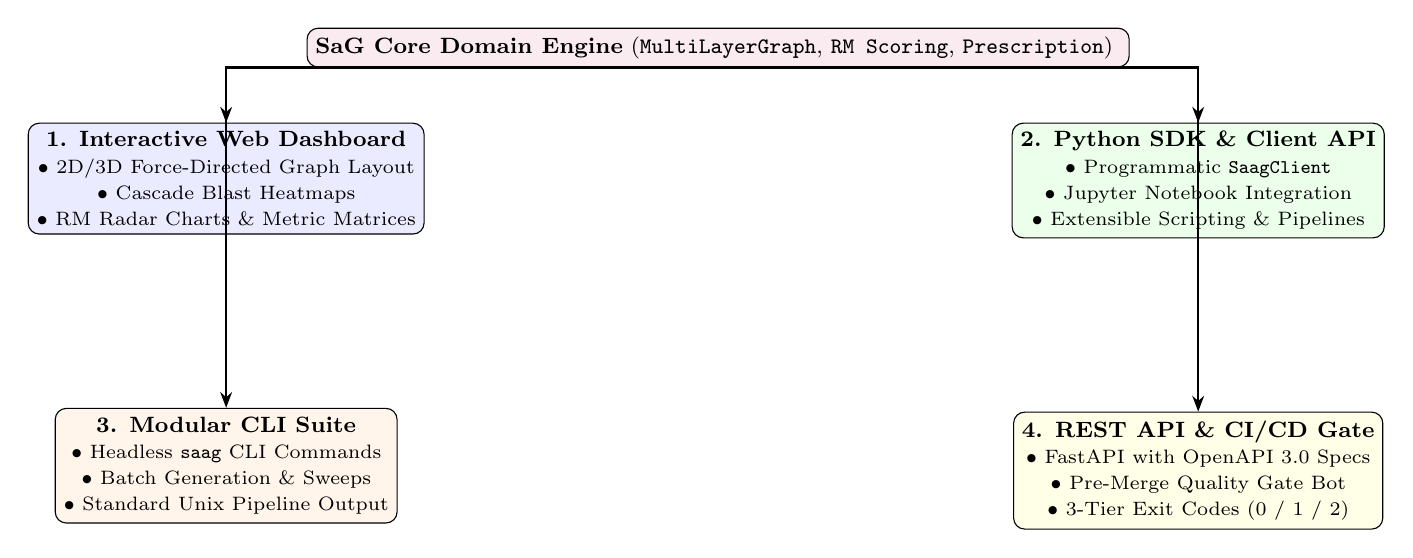
\begin{tikzpicture}[
    box/.style={draw, rounded corners, align=center, font=\footnotesize, inner sep=3pt},
    arr/.style={-{Stealth[length=2mm]}, thick},
    node distance=5mm and 6mm
]
\node[box, fill=purple!8, minimum width=9.5cm] (engine) {
    \textbf{SaG Core Domain Engine} (\texttt{MultiLayerGraph}, \texttt{RM Scoring}, \texttt{Prescription})
};

\node[box, fill=blue!8, below left=7mm and -15mm of engine, minimum width=4.3cm] (web) {
    \textbf{1. Interactive Web Dashboard} \\
    \scriptsize $\bullet$ 2D/3D Force-Directed Graph Layout \\
    \scriptsize $\bullet$ Cascade Blast Heatmaps \\
    \scriptsize $\bullet$ RM Radar Charts \& Metric Matrices
};

\node[box, fill=green!8, below right=7mm and -15mm of engine, minimum width=4.3cm] (sdk) {
    \textbf{2. Python SDK \& Client API} \\
    \scriptsize $\bullet$ Programmatic \texttt{SaagClient} \\
    \scriptsize $\bullet$ Jupyter Notebook Integration \\
    \scriptsize $\bullet$ Extensible Scripting \& Pipelines
};

\node[box, fill=orange!8, below=22mm of web, minimum width=4.3cm] (cli) {
    \textbf{3. Modular CLI Suite} \\
    \scriptsize $\bullet$ Headless \texttt{saag} CLI Commands \\
    \scriptsize $\bullet$ Batch Generation \& Sweeps \\
    \scriptsize $\bullet$ Standard Unix Pipeline Output
};

\node[box, fill=yellow!10, below=22mm of sdk, minimum width=4.3cm] (api) {
    \textbf{4. REST API \& CI/CD Gate} \\
    \scriptsize $\bullet$ FastAPI with OpenAPI 3.0 Specs \\
    \scriptsize $\bullet$ Pre-Merge Quality Gate Bot \\
    \scriptsize $\bullet$ 3-Tier Exit Codes (0 / 1 / 2)
};

\draw[arr] (engine.south) -| (web.north);
\draw[arr] (engine.south) -| (sdk.north);
\draw[arr] (engine.south) -| (cli.north);
\draw[arr] (engine.south) -| (api.north);
\end{tikzpicture}
\caption{Multi-modal interaction ecosystem of the Software-as-a-Graph framework.}
\label{fig:tool_interfaces}
\end{figure}

\subsubsection{Interactive Web Dashboard and Visual Graph Explorer}
For software architects and reliability engineers, SaG provides an interactive web dashboard developed in Next.js and React, complemented by a zero-dependency self-contained HTML dashboard generator (\texttt{saag.visualization.dashboard}). The visual explorer provides:
\begin{itemize}
    \item \textbf{Dynamic Topology Visualization:} Interactive 2D/3D force-directed network graphs rendering nodes, topics, brokers, and dependencies with color-coded severity tiers.
    \item \textbf{Cascade Heatmaps:} Visual overlays depicting simulated blast radii under single- and multi-node failure injection.
    \item \textbf{RM Diagnostic Radar Charts:} Multi-axis radial plots comparing Fault Tolerance, Availability, and Maintainability across subsystems.
    \item \textbf{Dependency Matrix and Triage Views:} Tabular cross-layer dependency matrices highlighting high-coupling hotspots and anti-pattern findings.
\end{itemize}

\subsubsection{Python SDK and Client API}
For systems researchers and data scientists, SaG exposes a native Python client library (\texttt{saag.client.SaagClient}) and pipeline orchestration interface (\texttt{saag.pipeline.Pipeline}). The SDK enables programmatic topology generation, metric extraction, counterfactual model mutation, and statistical validation within Jupyter notebooks and automated simulation testbeds:
\begin{verbatim}
from saag.client import SaagClient
client = SaagClient.from_config("config/saag.yaml")
graph = client.model.import_topology("data/scenarios/s01_av.json")
diagnosis = client.diagnose.evaluate(graph, layer="app")
print(f"Critical components: {diagnosis.get_critical_nodes()}")
prescription = client.prescribe.run_verified(graph, margin=1.0)
\end{verbatim}

\subsubsection{Command-Line Interface (CLI) Suite}
For automated batch execution and headless cluster sweeps, SaG offers a modular command-line suite:
\begin{itemize}
    \item \texttt{saag model}: Ingests architecture manifests and populates graph repositories.
    \item \texttt{saag diagnose}: Computes CQP, RM attributions, and executes anti-pattern detectors.
    \item \texttt{saag prescribe}: Compiles and counterfactually verifies refactoring candidates.
    \item \texttt{saag simulate}: Runs discrete-event cascade simulations with configurable seed sweeps.
    \item \texttt{saag validate}: Correlates structural predictions against ground-truth cascade outcomes.
\end{itemize}

\subsubsection{RESTful API Service}
SaG includes a production-ready asynchronous web service built with FastAPI (\texttt{api/main.py}). The API exposes full OpenAPI 3.0 documentation, enabling external engineering platforms (e.g., Jenkins, GitLab CI, GitHub Actions) to trigger analysis and retrieve serialized JSON diagnostic payloads over HTTP.

\subsection{DevOps Integration and CI/CD Quality Gating}
\label{sec:cicd_gating}

To prevent architectural regression during continuous system evolution, SaG's diagnostic engine is packaged as an automated quality gate for continuous integration workflows.

\subsubsection{Regression Semantics: Absolute vs.\ Delta-Aware Gating}
\label{sec:cicd:semantics}

The gate supports two operational evaluation modes:
\begin{itemize}
    \item \textbf{Absolute Gating:} Evaluates the complete system topology against global thresholds. However, mature industrial software systems frequently maintain accepted, intentional architectural debt. Under absolute gating on our benchmark corpus, the presence of legacy \texttt{CRITICAL} or \texttt{HIGH} findings triggers \textbf{Exit Code 2 (Block) on all eight scenarios} (Section~\ref{sec:results:performance}). This demonstrates that absolute gating is too rigid for iterative development.
    \item \textbf{Delta-Aware Gating (Design):} Compares the candidate pull-request topology against the target branch merge-base, blocking only \emph{newly introduced} anti-patterns or worsening severity classifications, while respecting signed \textbf{waiver registers} for risk-accepted legacy debt.
\end{itemize}

\subsubsection{Three-Tier Exit-Code Protocol}
\label{sec:cicd:protocol}

The quality gate communicates verdicts to CI runners via a standardized three-tier exit-code protocol:
\begin{itemize}
    \item \textbf{Exit Code 0 (Pass):} No critical architectural anti-patterns detected; build is cleared for deployment.
    \item \textbf{Exit Code 1 (Warning):} Non-critical \texttt{MEDIUM}-severity smells detected; build passes with advisory warnings posted to developers.
    \item \textbf{Exit Code 2 (Block):} Severe \texttt{CRITICAL} or \texttt{HIGH} anti-patterns detected; deployment pipeline is halted.
\end{itemize}

\section{Empirical Application in Realistic Scenarios}
\label{sec:empirical_application}

\subsection{Benchmark Scenarios and Real-World Corpora}
\label{sec:exp:scenarios}

To evaluate SaG across diverse system domains and scales, we employ an evaluation corpus comprising eight synthetic benchmark scenarios (Table~\ref{tab:scenarios}) and three architectures transcribed from open-source systems.

\begin{table}[htbp]
\centering
\footnotesize
\setlength{\tabcolsep}{3.5pt}
\caption{Benchmark Scenario Scales and Topological Dimensions.}
\label{tab:scenarios}
\begin{tabular}{lrrrrrr}
\toprule
\textbf{Scenario} & \textbf{Applications} & \textbf{Libraries} & \textbf{Topics} & \textbf{Brokers} & \textbf{Nodes} & \textbf{Total Edges ($|E|$)} \\
\midrule
S01 Autonomous Vehicle & 80 & 20 & 40 & 4 & 8 & 797 \\
S02 IoT Smart City & 200 & 10 & 80 & 6 & 30 & 1322 \\
S03 Financial Trading & 60 & 18 & 35 & 5 & 6 & 580 \\
S04 Healthcare & 50 & 12 & 25 & 3 & 8 & 400 \\
S05 Hub-and-Spoke & 70 & 25 & 30 & 2 & 12 & 797 \\
S06 Microservices Mesh & 90 & 30 & 45 & 6 & 15 & 680 \\
S07 Hyper-Scale Enterprise & 300 & 50 & 120 & 10 & 40 & 3245 \\
S08 Tiny Regression & 12 & 4 & 8 & 2 & 3 & 101 \\
\midrule
\textbf{Transcribed Real-World Topologies} & & & & & & \\
Autoware.Universe (ROS~2/DDS) & 32 & 10 & 24 & 3 & 6 & 284 \\
Train-Ticket (Microservices) & 41 & 8 & 30 & 3 & 8 & 342 \\
Cloud IoT Mesh (MQTT) & 22 & 8 & 20 & 4 & 6 & 195 \\
\bottomrule
\end{tabular}
\end{table}

Scenarios S01--S08 span six architectural domains ranging from 29 to 520 vertices (12 to 300 applications). Scenarios S01--S07 evaluate prescriptive refactoring; S08 is retained as a regression smoke test. To evaluate real-world validity, we include three architectures transcribed from production open-source systems: \textbf{Autoware.Universe} (the leading open-source ROS~2/DDS autonomous driving stack), the \textbf{Train-Ticket} microservices benchmark, and a \textbf{Cloud IoT Mesh} modeled on an industrial e-commerce and MQTT telemetry gateway.

\subsection{Research Questions and Evaluation Protocol}
\label{sec:exp:protocol}

Our empirical evaluation addresses five central research questions:
\begin{itemize}
    \item \textbf{RQ1 (Diagnostic Ranking Efficacy):} How does the RM composite's rank correlation with cascade failure impact compare to structural baselines (betweenness, degree centrality)?
    \item \textbf{RQ2 (Catalog Discrimination and Calibration):} How does the anti-pattern catalog perform on synthetic versus real-world topologies, and what explains its implication rate?
    \item \textbf{RQ3 (Attribution Validity and Substrate Adequacy):} Does the Availability dimension carry genuine signal on the application layer, and how does node stratification resolve Simpson's paradox?
    \item \textbf{RQ4 (Prescriptive Refactoring Efficacy and Operator Survival):} Does the closed-loop prescriptive engine achieve measurable reductions in cascade impact and System Risk Index, and how do individual mutation operators survive counterfactual verification?
    \item \textbf{RQ5 (Tool Performance and Verification Latency):} What is the execution latency of diagnostic gating and counterfactual verification across system scales?
\end{itemize}

\paragraph{Evaluation Protocol and Metrics.}
\begin{itemize}
    \item \textbf{Detection Metrics:} Spearman rank correlation $\rho(Q, I_{\text{comp}})$, Cohen's $\kappa$, Normalized Discounted Cumulative Gain ($\mathrm{NDCG@10}$), Top-10 overlap, precision, recall, and $F_1$ against discrete-event simulation ground truth $I_{\text{comp}}(v)$.
    \item \textbf{Prescriptive Metrics (Primary):} Mean fractional cascade-impact reduction on the fully mutated graph: $\overline{\Delta I}_{\text{policy}} = \mathrm{mean}_v\,[I(v) - I'(v)]/I(v)$, measured by the independent cascade simulator.
    \item \textbf{Prescriptive Metrics (Secondary):} System Risk Index change $\Delta\mathrm{SRI} = \mathrm{SRI}_{\text{baseline}} - \mathrm{SRI}_{\text{mutated}}$, serving as an internal consistency check.
    \item \textbf{Verification Parameters:} Propagation thresholds $\Theta = \{0.1, 0.2, 0.5\}$, random seeds $S = \{42, 123, 456\}$, and noise rejection margin $\kappa = 1.0$.
\end{itemize}

\subsection{Diagnostic Ranking Efficacy and Predictor Saturation (RQ1)}
\label{sec:results:detection}

Table~\ref{tab:detection_results} summarizes diagnostic performance at the application layer across all eight scenarios. Table~\ref{tab:predictor_comparison} compares the RM composite against single-metric baselines.

\begin{table}[htbp]
\centering
\footnotesize
\setlength{\tabcolsep}{3pt}
\caption{Diagnostic detection validation (app layer) against simulation ground truth $I_{\text{comp}}(v)$.}
\label{tab:detection_results}
\begin{tabular}{lrrrrrrrr}
\toprule
\textbf{Scenario} & $n$ & $\rho(Q, I)$ & $F_1$ & \textbf{Top-5} & \textbf{Catalog P} & \textbf{Catalog R} & \textbf{Implicated \%} & \textbf{Gate (s)} \\
\midrule
S01 Autonomous Vehicle & 80 & 0.457 & 0.600 & 0.40 & 0.244 & 0.950 & 97.5\% & 0.59 \\
S02 IoT Smart City & 200 & 0.718 & 0.780 & 0.40 & 0.310 & 0.880 & 71.0\% & 0.56 \\
S03 Financial Trading & 60 & 0.365 & 0.667 & 1.00 & 0.237 & 0.933 & 98.3\% & 0.40 \\
S04 Healthcare & 50 & 0.451 & 0.538 & 0.60 & 0.213 & 0.769 & 94.0\% & 0.16 \\
S05 Hub-and-Spoke & 70 & 0.466 & 0.611 & 0.80 & 0.257 & 1.000 & 100.0\% & 0.92 \\
S06 Microservices Mesh & 90 & 0.405 & 0.565 & 0.40 & 0.261 & 1.000 & 97.8\% & 0.35 \\
S07 Hyper-Scale Enterprise & 300 & 0.480 & 0.627 & 0.20 & 0.251 & 1.000 & 99.7\% & 20.98 \\
S08 Tiny Regression & 12 & 0.538 & 0.333 & 0.60 & 0.250 & 1.000 & 100.0\% & 0.01 \\
\midrule
\textbf{Mean} & --- & \textbf{0.485} & \textbf{0.590} & \textbf{0.550} & \textbf{0.253} & \textbf{0.942} & \textbf{94.8\%} & \textbf{3.00} \\
\bottomrule
\end{tabular}
\end{table}

\begin{table}[htbp]
\centering
\small
\caption{Predictor Comparison (App Layer, Mean over 8 Scenarios). Structural predictors saturate around comparable ranking quality.}
\label{tab:predictor_comparison}
\begin{tabular}{lrrrr}
\toprule
\textbf{Predictor} & $\rho$ & \textbf{Cohen's $\kappa$} & \textbf{NDCG@10} & \textbf{Top-10} \\
\midrule
$Q(v)$ composite (RM) & 0.4850 & 0.4514 & 0.8295 & 0.5875 \\
Betweenness & 0.4346 & 0.4139 & \textbf{0.8592} & \textbf{0.6250} \\
Degree Centrality & \textbf{0.5187} & \textbf{0.4792} & 0.8214 & 0.5625 \\
\bottomrule
\end{tabular}
\end{table}

\paragraph{Predictor Saturation.}
As Table~\ref{tab:predictor_comparison} illustrates, all three predictors saturate around comparable performance: degree centrality leads slightly on $\rho$ ($0.519$) and $\kappa$ ($0.479$), betweenness leads on $\mathrm{NDCG@10}$ ($0.859$) and Top-10 overlap ($0.625$), while the RM composite $Q(v)$ achieves balanced ranking ($\rho = 0.485$, $\mathrm{NDCG@10} = 0.830$). Under a Wilcoxon paired signed-rank test across scenarios, $Q(v)$ versus degree centrality yields $p = 0.945$ (paired $t$-test, $p = 0.465$); head-to-head, $Q(v)$ attains higher correlation in \textbf{five of eight} scenarios. This empirical saturation demonstrates that no single scalar predictor dominates. Consequently, the primary value of the RM model is not superior ranking accuracy, but rather its **deterministic, role-attributed quality decomposition** into actionable Fault Tolerance, Availability, and Maintainability dimensions.

\subsection{Catalog Calibration on Synthetic vs.\ Transcribed Topologies (RQ2)}
\label{sec:results:calibration}
\label{sec:results:realworld}

On the generated benchmark scenarios, the anti-pattern catalog exhibits high screening recall ($0.942$) and low precision ($0.253$), implicating an average of $94.8\%$ of components with chance-level agreement ($\kappa = -0.0022$). As detailed in Section~\ref{sec:catalog:coverage}, this is driven by finding scope: $98.4\%$ of findings are edge-scoped (\texttt{BOTTLENECK\_EDGE} and \texttt{QOS\_MISMATCH}), which implicate all connected endpoints.

To assess whether this is an artifact of synthetic topology generation, we evaluated the catalog across the three transcribed real-world open-source systems over five simulation seeds (Table~\ref{tab:realworld}).

\begin{table}[htbp]
\centering
\footnotesize
\setlength{\tabcolsep}{4pt}
\caption{Catalog behavior on generated versus transcribed topologies (System Layer, 5 seeds). The catalog discriminates effectively on real-world architectures.}
\label{tab:realworld}
\begin{tabular}{lrr}
\toprule
\textbf{Measure} & \textbf{Generated} ($n=40$) & \textbf{Transcribed} ($n=15$) \\
\midrule
Cohen's $\kappa$          & $-0.036 \pm 0.049$ & $\mathbf{+0.296 \pm 0.100}$ \\
Precision                 & $0.237 \pm 0.014$  & $\mathbf{0.402 \pm 0.060}$ \\
Recall                    & $0.887 \pm 0.059$  & $0.861 \pm 0.105$ \\
$F_1$                     & $0.374 \pm 0.022$  & $\mathbf{0.545 \pm 0.061}$ \\
Components Implicated     & $93.7\% \pm 3.2$   & $\mathbf{56.3\% \pm 9.8}$ \\
\bottomrule
\end{tabular}
\end{table}

On transcribed architectures, chance-corrected agreement rises to $\mathbf{\kappa = +0.296}$ (fair agreement), precision increases by two-thirds to $0.402$, and the component implication rate drops from $93.7\%$ to $56.3\%$ ($21.3\%$ in Autoware, $18.3\%$ in Cloud Mesh, $14.4\%$ in Train-Ticket). This confirms that the catalog's indiscriminate behavior is largely an artifact of the dense uniform edge distributions in synthetic generators, whereas modular real-world architectures provide natural structural boundaries where anti-patterns discriminate effectively.

\subsection{Attribution Validity and Substrate Adequacy (RQ3)}
\label{sec:results:attribution}

\paragraph{Availability Degeneracy on Application Layer.}
At the application layer, the \texttt{SPOF} detector scores $F_1 = 0.0$ in \textbf{all eight scenarios}, predicting zero articulation points in six scenarios. Because $A(v)$ carries $0.64$ of $R(v)$'s weight, half of the composite score on this layer is computed over a near-constant substrate. This confirms Section~\ref{sec:model:substrate}'s substrate adequacy theorem: Availability metrics must be evaluated on Middleware or System layer projections where brokers and compute nodes create genuine physical bottlenecks.

\paragraph{Reconciling Prior Conference Findings.}
Our preliminary conference study \citep{yigit2025graph} reported $\rho = 0.94$ on a 10-application system validated against reachability loss. That earlier result shared its computational substrate with the predictor (both computed on the undirected application graph) and examined a topology with deliberate cut-vertices. This paper evaluates an independent discrete-event cascade oracle on directed dependency graphs across up to 300 applications, revealing the realistic saturation baseline ($\rho \approx 0.485$).

\paragraph{Simpson's Paradox in Multi-Type Pooling.}
When all five entity types are pooled at the system layer, the aggregate correlation collapses to $\rho = 0.028$, even though within-type strata show strong positive correlation (Application $0.503$, Broker $0.395$, Node $0.142$). This is a textbook instance of Simpson's paradox arising from baseline score offsets between entity types, demonstrating that stratified evaluation is a mandatory requirement for heterogeneous software graphs.

\subsection{Prescriptive Refactoring Performance and Operator Survival (RQ4)}
\label{sec:results:prescriptive}

Table~\ref{tab:prescriptive_results} details the closed-loop refactoring results across all seven prescriptive scenarios, and Table~\ref{tab:operator_results} breaks down admission by mutation operator.

\begin{table}[htbp]
\centering
\footnotesize
\setlength{\tabcolsep}{2.5pt}
\caption{Prescriptive refactoring performance under per-edit counterfactual verification.}
\label{tab:prescriptive_results}
\begin{tabular}{lrrrrrr}
\toprule
\textbf{Scenario} & $\overline{\Delta I}_{\text{policy}}$ & $\Delta\mathrm{SRI}$ & \textbf{Cand.} & \textbf{Adm.} & \textbf{Rej.} & \textbf{Adm.\ \%} \\
 & \scriptsize(primary, oracle) & \scriptsize(secondary, RM) & & & & \\
\midrule
S01 Autonomous Vehicle & $+0.0161$ & +0.0086 & 156 & 45 & 111 & 28.8\% \\
S02 IoT Smart City & $+0.0822$ & \textbf{+0.0461} & 391 & 297 & 94 & 76.0\% \\
S03 Financial Trading & $\mathbf{-0.0689}$ & +0.0108 & 125 & 22 & 103 & 17.6\% \\
S04 Healthcare & $\mathbf{+0.1894}$ & +0.0109 & 99 & 36 & 63 & 36.4\% \\
S05 Hub-and-Spoke & $+0.0236$ & +0.0115 & 127 & 107 & 20 & 84.3\% \\
S06 Microservices Mesh & $\mathbf{-0.0015}$ & +0.0097 & 163 & 142 & 21 & 87.1\% \\
S07 Hyper-Scale Enterprise & $+0.0060$ & \textbf{+0.0171} & 528 & 479 & 49 & 90.7\% \\
\midrule
\textbf{Mean / Total} & \textbf{+0.0352} & --- & \textbf{1589} & \textbf{1128} & \textbf{461} & \textbf{71.0\%} \\
\textbf{Scenarios Improved} & \textbf{5 / 7} & \textbf{7 / 7} & & & & \\
\bottomrule
\end{tabular}
\end{table}

\begin{table}[htbp]
\centering
\footnotesize
\setlength{\tabcolsep}{3.5pt}
\caption{Candidate Generation vs.\ Verified Admission by Refactoring Operator.}
\label{tab:operator_results}
\begin{tabularx}{\textwidth}{lrrr>{\raggedright\arraybackslash}X}
\toprule
\textbf{Refactoring Operator} & \textbf{Candidates} & \textbf{Admitted} & \textbf{Survival Rate} & \textbf{Primary Structural Target} \\
\midrule
\textbf{Physical Anti-Affinity Reallocation} & 1188 & \textbf{923} & \textbf{77.7\%} & Single points of failure, co-location \\
\textbf{Transport QoS Contract Hardening} & 69 & \textbf{40} & \textbf{58.0\%} & Volatile transport contracts on topics \\
\textbf{Logical Topic Splitting} & 332 & \textbf{165} & \textbf{49.7\%} & High-fan-out message channels, hubs \\
\midrule
\textbf{Total} & \textbf{1589} & \textbf{1128} & \textbf{71.0\%} & --- \\
\bottomrule
\end{tabularx}
\end{table}

\paragraph{Key Prescriptive Findings.}
\begin{enumerate}
    \item \textbf{Verification Yield:} Across 1589 compiled candidates, \textbf{1128 edits ($71.0\%$)} survive counterfactual verification, while 461 edits ($29.0\%$) are filtered out because they fail to clear simulator noise.
    \item \textbf{Operator Survival:} Physical anti-affinity reallocation demonstrates the highest survival rate ($77.7\%$), followed by transport QoS hardening ($58.0\%$) and topic splitting ($49.7\%$).
    \item \textbf{Oracle-Measured Impact Reduction:} Under the independent cascade oracle, five of seven scenarios achieve net cascade-impact reduction (mean $+3.52\%$, reaching $+18.9\%$ in Healthcare). Two scenarios regress slightly under joint composition (S03 $-6.9\%$, S06 $-0.15\%$), demonstrating that individually verified edits can interact sub-additively.
    \item \textbf{Internal Risk Index ($\Delta\mathrm{SRI}$):} All seven scenarios achieve positive $\Delta\mathrm{SRI}$ gains (Wilcoxon $W=0, p=0.0156$). However, because $\Delta\mathrm{SRI}$ evaluates the same RM dimensions used to compile candidates, we treat the independent oracle's $+3.52\%$ impact reduction as the definitive headline measure.
\end{enumerate}

\subsection{Tool Performance, Scalability, and Latency (RQ5)}
\label{sec:results:performance}

\begin{enumerate}
    \item \textbf{Diagnostic Pipeline Execution Latency:} The complete diagnostic pipeline (graph parsing, CQP computation, RM attribution, and 18 active detectors) executes in \textbf{0.01~s to 20.98~s} across the corpus (Table~\ref{tab:detection_results}). The 18 detectors run in under \textbf{0.2~s total}; overhead is dominated by base shortest-path and centrality calculations.
    \item \textbf{\texttt{DEEP\_PIPELINE} Bounding:} Unconstrained path enumeration in the \texttt{DEEP\_PIPELINE} detector generated 247,761 paths on small fixtures and hung on enterprise graphs. Excluding it restored sub-second execution across small-to-medium scenarios.
    \item \textbf{Prescriptive Verification Throughput:} The complete prescriptive sweep across seven scenarios (comprising 14,301 discrete-event simulation sweeps) executed in \textbf{2~h 47~min} on a 20-core workstation using \texttt{MemoryRepository}, confirming the computational feasibility of nightly automated refactoring verification.
\end{enumerate}

\section{Community Importance and Lessons Learnt}
\label{sec:community_and_lessons_learnt}

In accordance with the guidelines of the SoSyM Tool Paper Call, this section explicitly articulates why the Software-as-a-Graph framework is important for the systems and modeling community, followed by five transferable lessons learnt from designing, building, testing, evaluating, and disseminating the tool.

\subsection{Importance for the Systems and Software Modeling Community}
\label{sec:community:importance}

\begin{enumerate}
    \item \textbf{Addressing the MDE Blind Spot for Asynchronous Pub--Sub Systems:} While Model-Driven Engineering has produced mature modeling languages and tools for synchronous RPC, component-connector monoliths, and embedded control loops (e.g., AADL, Palladio, SysML), asynchronous publish--subscribe architectures have remained a significant blind spot. Contemporary cyber-physical systems, autonomous vehicles (ROS~2/DDS), and IoT clouds rely heavily on topic-based pub--sub middleware. SaG provides the modeling community with a formalized, open-source metamodel, multi-layer projection rules, and quality attribution framework tailored specifically to the semantics of asynchronous message-passing systems.
    \item \textbf{A Standardized, Reproducible Experimental Benchmark Testbed:} A recurring obstacle in software architecture and modeling research is the scarcity of open, diverse, and realistic benchmark models. SaG delivers an open corpus of eight multi-scale benchmark topologies (spanning autonomous driving, smart cities, financial trading, healthcare, and microservices) alongside three transcribed real-world open-source architectures (Autoware.Universe, Train-Ticket, Cloud IoT Mesh). This corpus, complete with declarative descriptors and discrete-event simulation oracles, establishes a shared experimental substrate for researchers developing new graph metrics, smell detectors, and model optimizers.
    \item \textbf{Reusable Catalog of Anti-Patterns and Refactoring Operators:} SaG formalizes nineteen architectural anti-patterns and three graph-mutation operators stated over native publish--subscribe constructs. By publishing complete metric formulas, detection algorithms, and mutation preconditions, SaG provides a modular specification that other MDE researchers can adopt, extend, or transcribe into other modeling formalisms (e.g., EMF/Ecore, AGG, Henshin).
    \item \textbf{Operationalizing International Quality Standards in Graph Models:} Many predictive modeling tools rely on ad-hoc scalar metrics or opaque neural networks. SaG demonstrates how international quality standards (\textbf{ISO/IEC 25010} and \textbf{ISO/IEC 25019}) can be operationalized deterministically over graph models, establishing an auditable bridge between source-code metrics (CQP) and macro-architectural risk.
\end{enumerate}

\subsection{Lessons Learnt Designing, Building, Testing, and Disseminating the Tool}
\label{sec:community:lessons}

\subsubsection{Lesson 1 (Designing): Metamodel Substrate Adequacy and Layer Awareness}
\textit{Architectural quality metrics are only as valid as the projection substrate on which they are evaluated.} 

A common design instinct in MDE is to define a structural metric (such as articulation-point membership for Single Points of Failure) and evaluate it across whatever graph model is available. In SaG, our initial design evaluated the complete RM composite at the application layer. However, because application-layer projections abstract away underlying middleware brokers and host nodes, topics often present redundant alternate paths, rendering cut-vertices structurally nonexistent ($F_1 = 0.0$ for SPOF detection across all eight scenarios). 

\textbf{Takeaway for tool designers:} Multi-level system models must formally specify the exact architectural layer on which each quality metric is mathematically well-posed. Discrete connectivity metrics must be evaluated on layers where physical mediation bottlenecks actually exist (e.g., Middleware and Infrastructure layers), rather than assuming that application-layer projections reflect global availability risks.

\subsubsection{Lesson 2 (Building): Dual Repositories for Counterfactual Model Transformation}
\textit{Graph databases are ideal for persistent exploration, but in-memory copy-on-write sandboxes are mandatory for high-throughput model verification.}

Initially, our tool prototype executed all graph operations directly against Neo4j via Cypher queries. While Neo4j provided excellent persistence, expressive graph queries, and visual debugging, using it for closed-loop refactoring verification created severe performance bottlenecks: executing thousands of speculative graph mutations, running cascade simulations, and rolling back state incurred severe disk I/O, network serialization, and transaction locking delays. 

\textbf{Takeaway for tool designers:} By adopting a hexagonal ports-and-adapters architecture around an abstract \texttt{IGraphRepository} port, we implemented a specialized \texttt{MemoryRepository}. This in-memory adapter uses vectorized adjacency lists and thread-safe copy-on-write branching, enabling isolated counterfactual mutation sweeps to execute in microseconds and completing 14,301 simulation sweeps in 2~h 47~min. Tool builders should cleanly separate persistent query stores from ephemeral, in-memory execution sandboxes.

\subsubsection{Lesson 3 (Testing): The ``Verify-Before-Transform'' Discipline}
\textit{Rule-based model refactoring cannot be trusted open-loop; candidate transformations must be counterfactually verified against dynamic failure cascades.}

In the model refactoring literature, transformation rules are typically assumed to improve system quality by definition (e.g., splitting a congested topic must reduce coupling). When we tested this assumption against our discrete-event cascade simulator, we discovered that \textbf{461 of 1589 compiled refactoring candidates ($29.0\%$)} failed verification: their measured cascade-impact reduction did not exceed stochastic seed noise, or they introduced subtle downstream congestion that exacerbated cascade reach. Furthermore, in two scenarios (S03 and S06), individually beneficial edits composed sub-additively into a net regression under joint application.

\textbf{Takeaway for tool designers:} In complex distributed architectures, static heuristic rules are insufficient to guarantee resilience. Refactoring tools must incorporate closed-loop counterfactual simulation or formal verification into the transformation pipeline, actively discarding plausible-looking edits that fail to demonstrate measurable dependability gains beyond noise.

\subsubsection{Lesson 4 (Evaluating): Explanatory Attribution vs.\ Scalar Centrality Ranking}
\textit{Multi-metric composite scores do not necessarily out-rank simple centralities; their true value lies in explainable, role-specific quality attribution.}

A foundational hypothesis in software metrics research is that multi-dimensional composite scores should significantly outperform simple graph centralities for predicting structural failure impact. Our empirical findings decisively qualify this assumption: across eight scenarios, degree centrality ($\rho = 0.519$), betweenness ($\mathrm{NDCG@10} = 0.859$), and the RM composite ($\rho = 0.485$, $\mathrm{NDCG@10} = 0.830$) saturate at statistically indistinguishable ranking quality (paired $p = 0.95$). 

\textbf{Takeaway for tool designers:} Modeling researchers should resist the urge to claim superior ranking accuracy where empirical evidence demonstrates saturation. Instead, the true value of domain-grounded modeling is \emph{explanatory attribution}: a scalar degree centrality cannot tell an engineer whether a component is critical due to deep cascade reach (Reliability Engineer), single-point-of-failure exposure (SRE), or high coupling debt (Software Architect). Grounding models in standardized, auditable quality taxonomies provides actionable engineering value that raw centralities cannot offer.

\subsubsection{Lesson 5 (Disseminating): Multi-Modal Ergonomics for Diverse Modeling Personas}
\textit{Tool adoption requires meeting diverse stakeholders in their native operational environments.}

During early dissemination of SaG, we observed that different engineering personas rejected tools that did not fit their established workflows. Systems architects preferred visual graph layouts, interactive heatmaps, and radar charts over raw data tables. Systems researchers and MDE modelers demanded scriptable Python APIs and Jupyter notebook integration for rapid experimentation. Conversely, DevOps engineers flatly rejected graphical interfaces, demanding headless CLI binaries with deterministic Unix exit codes (0/1/2) that could run within sub-second pre-merge CI/CD quality gates.

\textbf{Takeaway for tool designers:} A modeling tool must provide synchronized multi-modal interaction interfaces: an interactive web dashboard for visual exploration, a programmatic Python SDK for research, and a headless CLI and REST API for continuous automated governance.

\section{Discussion and Tool Availability}
\label{sec:discussion}

\subsection{Threats to Validity}
\label{sec:disc:threats}

\begin{itemize}
    \item \textbf{Construct Validity --- Circularity of Whole-Policy Gating:} While the Level 1 per-edit filter utilizes an independent cascade oracle, the Level 2 whole-policy gate evaluates $\Delta\mathrm{SRI}$, which reweights the same RM dimensions used to compile candidates. This is why Section~\ref{sec:results:prescriptive} treats the oracle-measured cascade reduction ($\overline{\Delta I}_{\text{policy}}$) as the primary outcome and $\Delta\mathrm{SRI}$ as an internal consistency check.
    \item \textbf{Construct Validity --- Substrate Adequacy:} As formalized in Section~\ref{sec:model:substrate}, discrete topological predicates (e.g., articulation points) collapse on projections lacking cut structures. Availability metrics must be evaluated on Middleware or Infrastructure projections where mediation bottlenecks are physically present.
    \item \textbf{Internal Validity --- Independence in Verification:} Decoupled in-memory graph sandboxing (\texttt{MemoryRepository}) guarantees that speculative graph mutations do not leak state into baseline graphs or cross-contaminate concurrent verification sweeps.
    \item \textbf{External Validity --- Synthetic vs.\ Real-World Generalization:} The eight core benchmark scenarios are synthetic generators. We mitigated this by evaluating three transcribed real-world open-source systems (Autoware.Universe, Train-Ticket, Cloud IoT Mesh), demonstrating that the catalog achieves substantial chance-corrected agreement ($\kappa = +0.296$) on realistic topologies.
    \item \textbf{Conclusion Validity --- Sample Size and Effect Significance:} The primary oracle-measured reduction ($+3.52\%$) across seven prescriptive scenarios does not achieve statistical significance under a two-sided Wilcoxon signed-rank test ($p = 0.219, n=7$). We report this effect descriptively and provide complete per-scenario distributions.
\end{itemize}

\subsection{Tool Availability, Reproducibility, and Open Science}
\label{sec:tool:availability}

In strict compliance with SoSyM's tool availability criteria, Software-as-a-Graph (SaG) is developed and maintained as an open-source, fully reproducible scientific software framework:

\begin{itemize}
    \item \textbf{Open-Source License:} SaG is released under the permissive **Apache License 2.0**, granting complete freedom for academic research, extension, and industrial adoption.
    \item \textbf{Source Code Repository:} The full source code---including the core `saag` domain engine, the `cli` suite, the `api` service, and the web visualization components---is publicly hosted on GitHub at \url{https://github.com/software-as-a-graph/software-as-a-graph}.
    \item \textbf{Persistent Archival and DOI:} The repository, benchmark scenario datasets, and experimental outputs are permanently archived on Zenodo with a persistent Digital Object Identifier (DOI), registered via \texttt{.zenodo.json}.
    \item \textbf{Package Distribution and Containerization:} SaG is packaged for Python $\ge 3.10$ via \texttt{pyproject.toml} and can be installed directly with standard package managers. For zero-configuration deployment, a complete multi-container environment is provided via \texttt{docker-compose.yml}, orchestrating the Neo4j 5.x graph database, the FastAPI backend, and the interactive web explorer.
    \item \textbf{Reproduction Package:} The repository contains an automated reproduction suite under \texttt{reproduce/}. Running the automated harness reproduces all numerical values, tables, and figures reported in Section~\ref{sec:empirical_application} from raw artifact JSONs.
\end{itemize}

\section{Conclusion and Future Work}
\label{sec:conclusion}

\subsection{Conclusion}
\label{sec:conclusion:summary}

This tool paper presented \textbf{Software-as-a-Graph (SaG)}, an open-source, extensible Model-Driven Engineering framework for graph-based architectural modeling, diagnostic quality analysis, and counterfactually verified refactoring of distributed publish--subscribe software systems. By formalizing a domain-specific, typed multigraph metamodel ($V, E, \tau_V, \tau_E, w_V, w_E$) across four architectural layers, SaG bridges source-level code metrics (CQP) with macro-architectural risk, evaluating system health against ISO/IEC 25010 and ISO/IEC 25019 standards and formalizing nineteen publish--subscribe architectural anti-patterns.

To remediate architectural technical debt, SaG implements a closed-loop prescriptive engine driven by three graph-mutation operators. Adopting a strict \textbf{``verify-before-transform''} discipline, the tool simulates candidate mutations within in-memory sandboxes against a discrete-event cascade oracle, admitting only edits whose risk reduction clears stochastic seed noise. SaG's hexagonal architecture features a dual-repository pattern that pairs persistent Neo4j storage with an ultra-fast in-memory repository (\texttt{MemoryRepository}), supporting multi-modal interfaces spanning interactive web dashboards, Python SDKs, modular CLIs, REST APIs, and automated CI/CD quality gates.

Evaluated across eight benchmark scenarios and three transcribed real-world open-source systems (Autoware.Universe, Train-Ticket, Cloud IoT Mesh), SaG demonstrates high diagnostic screening sensitivity, superior discrimination on real-world modular architectures ($\kappa = +0.296$), a $71.0\%$ refactoring admission rate, and sub-second diagnostic gating latency. Crucially, we synthesize five transferable lessons learnt spanning metamodel substrate adequacy, in-memory sandboxing, simulation-in-the-loop verification, explanatory attribution versus ranking saturation, and multi-modal tool ergonomics to inform future tool builders in the systems modeling community.

\subsection{Future Work}
\label{sec:conclusion:future_work}

We identify several promising avenues for future tool evolution:
\begin{enumerate}
    \item \textbf{Layer-Aware Automated Availability Metrics:} Implementing multi-layer path analysis to automatically evaluate Availability predicates on Middleware or Infrastructure projections where cut structures are physically present.
    \item \textbf{Search-Based Multi-Objective Optimization (SBSE):} Expanding the current rule-based candidate compiler into a hybrid multi-objective search algorithm (e.g., NSGA-II) that optimizes failure impact, hardware migration cost, and network bandwidth under budget constraints.
    \item \textbf{Combinatorial Subset Verification:} Replacing the current greedy all-admitted policy gate with forward-selection subset verification to prevent sub-additive compositional regressions.
    \item \textbf{External Tool Benchmarking:} Executing comparative evaluations against general-purpose architectural smell detectors (e.g., Arcan, Designite) running over projected dependency graphs.
    \item \textbf{Automated Model Ingestion from IDLs and Traces:} Developing automated model extractors that directly parse ROS~2 package manifests, DDS XML QoS profiles, and Kafka topic definitions into SaG multigraphs.
    \item \textbf{LLM-Assisted Refactoring Implementation:} Integrating large language models with SaG's verified graph mutation blueprints to automatically synthesize infrastructure-as-code diffs (Kubernetes manifests, Docker Compose files) for immediate deployment.
\end{enumerate}


\section*{Declarations}

\paragraph{Funding:} This work was supported in part by the Scientific and Technological Research Council of T\"urkiye (T\"UB\.ITAK), grant number [GRANT-NUMBER].

\paragraph{Competing Interests:} The authors declare that they have no competing financial or non-financial interests that are directly or indirectly related to the work submitted for publication.

\paragraph{Related Submissions and Overlap Disclosure:} A companion manuscript by the same authors, \emph{Software-as-a-Graph: A Static System Analysis Framework for Pre-Deployment Quality Gating and Failure Simulation of Publish-Subscribe Middleware}, is currently under review at another journal. The two submissions share three research artifacts---the heterogeneous graph schema, the benchmark scenario corpus, and the discrete-event cascade simulator---and are otherwise disjoint. That manuscript contributes the learned Graph Neural Network pathway for failure-impact prediction and its evaluation; this manuscript contributes the deterministic Diagnostic Pathway, the Code Quality Penalty, the nineteen-pattern anti-pattern catalog, the prescriptive refactoring compiler, the counterfactual verification engine, and the CI/CD quality gate. No result, table, or figure appears in both. We disclose this so the editor can assess the overlap directly.

\paragraph{Data Availability:} All scenario topologies, generator configurations, result artifacts, seeds, and execution logs supporting the findings of this study are available in the replication package archived at [REPOSITORY-URL], persistent identifier \texttt{[TODO(DOI): mint a Zenodo DOI before submission]}. The two entry points that regenerate this paper's tables are:
\begin{verbatim}
PYTHONPATH=. python reproduce/detection_validation.py --layer app \
    --output results/detection_validation_app.json
PYTHONPATH=. python reproduce/run_prescribe_all.py --kappa 1.0
\end{verbatim}
The first regenerates Tables~\ref{tab:detection_results} and \ref{tab:predictor_comparison}; the second regenerates Tables~\ref{tab:prescriptive_results} and \ref{tab:operator_results}. The prescriptive sweep takes approximately 2\,h 47\,min on 20 cores.

\paragraph{Author Contributions:} [To be completed via the submission interface, per the journal's Submitting Declarations requirements.]

\paragraph{Ethics Approval:} Not applicable.


\bibliographystyle{plainnat}
\bibliography{refs}

\end{document}
